% =====================================================================
%  WCCM 2026 / ECCOMAS — MS090E, 22 July 2026.
%  PAPER-FAITHFUL deck: follows the Frontiers in Materials 2025 paper
%  (and the English slides 27-44 of nishioka_progress_20260114.pptx).
%  Extension (architecture sweep / variants) appears ONLY as a brief
%  outlook teaser — co-author-safe, per supervisor's instruction.
%  Build: latexmk -pdf wccm_beamer_paper.tex  (needs biber)
% =====================================================================
\documentclass[aspectratio=169,12pt]{beamer}

% =====================================================================
%  Clean, thesis-matching look: NO metropolis. Serif (Times via newtx),
%  understated navy accent, plain frame title with a thin rule, no colour
%  bars or progress bar — mirrors the master-thesis document style.
% =====================================================================
\usetheme{default}
\setbeamertemplate{navigation symbols}{}

\usefonttheme{professionalfonts}
\usepackage[T1]{fontenc}
\usepackage[utf8]{inputenc}
\usepackage{newtxtext,newtxmath}
\usepackage[protrusion=true,expansion=true]{microtype}

\usepackage{booktabs}
\usepackage{amsmath,amssymb}
\usepackage{graphicx}
\usepackage{xcolor}
\usepackage{tikz}
\usetikzlibrary{positioning,arrows.meta}
\usepackage{array}

\usepackage[style=numeric-comp,sorting=none,backend=biber,maxnames=2,giveninits=true]{biblatex}
\addbibresource{refs_submission.bib}
\renewcommand*{\bibfont}{\scriptsize}

% understated academic palette (thesis-like)
\definecolor{accent}{RGB}{20,43,84}      % deep navy
\definecolor{accentlt}{RGB}{225,229,238}
\definecolor{alertred}{RGB}{150,28,28}
\definecolor{okgreen}{RGB}{27,94,32}
\AtEveryCite{\scriptsize\color{accent}}

\setbeamercolor{structure}{fg=accent}
\setbeamercolor{title}{fg=accent}
\setbeamercolor{frametitle}{fg=accent,bg=}
\setbeamercolor{normal text}{fg=black!90}
\setbeamercolor{alerted text}{fg=alertred}
\setbeamercolor{example text}{fg=okgreen}
\setbeamercolor{block title}{fg=accent,bg=accentlt}
\setbeamercolor{block body}{bg=accentlt!40}
\setbeamercolor{block title alerted}{fg=white,bg=alertred}
\setbeamercolor{block title example}{fg=white,bg=okgreen}
\setbeamerfont{title}{series=\bfseries}
\setbeamerfont{frametitle}{series=\bfseries,size=\large}
\setbeamertemplate{blocks}[rounded][shadow=false]
\setbeamertemplate{itemize item}{\small\textbullet}
\setbeamertemplate{itemize subitem}{\scriptsize--}

% plain serif frame title with a thin navy rule beneath (no colour bar)
\setbeamertemplate{frametitle}{%
  \vskip0.7em%
  {\usebeamerfont{frametitle}\usebeamercolor[fg]{frametitle}\insertframetitle\par}%
  \vskip2pt{\color{accent}\hrule height 0.5pt}\vskip2pt}

% tiny source-attribution footer (very light, bottom). Our own Frontiers paper
% is attributed here, NOT cited as prior work in-text.
\setbeamertemplate{footline}{%
  \hbox{}\vspace{1pt}%
  \hbox to \paperwidth{\hskip2.5mm
    {\tiny\color{gray!60!black} Nishioka \textit{et al.}, Front.\ Mater.\ \textbf{12}:1652484 (2025)}%
    \hfill
    {\tiny\color{gray!60!black}\insertframenumber}\hskip2.5mm}%
  \vspace{2.5pt}}

% pympress speaker notes: build a notes PDF (slide | notes side-by-side) with
%   latexmk -jobname=wccm_beamer_paper_notes -usepretex='\def\NOTESBUILD{}' ...
% The plain build leaves \note{} invisible, so wccm_beamer_paper.pdf stays clean.
\ifdefined\NOTESBUILD
  \usepackage{pgfpages}
  \setbeameroption{show notes on second screen=right}
\fi

\graphicspath{{figures_paper/}{../results/}{figures/}}
\newcommand{\best}[1]{{\color{okgreen}\textbf{#1}}}

\title{Development of a Defect Estimation Method for CFRP Interstage
Structures with Holes using Finite Element Analysis and Graph Neural Networks}
\author[K.\ Nishioka et al.]{\underline{Keisuke Nishioka}\inst{1} \and Yuta Kojima\inst{2}
\and Toshiya Saito\inst{3} \and Masahito Washiya\inst{3}
\and Kosuke Kawakami\inst{3} \and Mayu Muramatsu\inst{4}}
\institute{\inst{1}Keio University, Sci.\ for Open \& Environ.\ Systems \quad
\inst{2}Nagoya University \\ \inst{3}JAXA, R\&D Directorate \quad
\inst{4}Keio University, Mech.\ Engineering}
\date{17th WCCM / ECCOMAS 2026, Munich \quad MS090E}

% =====================================================================
\begin{document}

{\setbeamertemplate{footline}{}\maketitle}
\note{Good morning. I am Keisuke Nishioka, from Keio University and Leibniz Universitaet Hannover, with co-authors at Nagoya University and JAXA. Today I show how we localize hidden delamination in perforated CFRP interstage structures using finite-element analysis and a graph neural network: 61\% macro-F1 from surface stress alone, and how we make it robust to measurement noise. About 15 minutes.}

% ---------------------------------------------------------------------
\begin{frame}{Outline}
\note{Quick roadmap: motivation and the DSPSS measurement, the method, the published results, the new noise-robustness work, and outlook. About 15 minutes.}
\begin{enumerate}
  \item Motivation \& measurement --- defects in CFRP, infrared stress (DSPSS)
  \item Method --- difference-normalized input \& a GAT on the FEM mesh
  \item Results --- 19-class 3-D localization (macro-F1 $61\%$)
  \item New: robustness to measurement noise (defect-free negatives)
  \item Outlook
\end{enumerate}
\end{frame}

% ---------------------------------------------------------------------
\begin{frame}{Contributions}
\note{State the three contributions up front, then dive in.}
\begin{columns}[T]
\begin{column}{0.56\textwidth}
\begin{enumerate}
  \item A \textbf{graph attention network} localizing 3-D delamination in
        \emph{perforated} CFRP interstages directly from FEM surface stress (DSPSS).
  \item \textbf{61\% macro-F1} over 19 classes (region $\times$ layer) from
        \emph{surface data only}, with defect false-negative rate $<3\%$.
  \item \textbf{Noise-robust} training (structured noise $+$ defect-free negatives)
        --- a step toward experimental infrared-stress data.
\end{enumerate}
\end{column}
\begin{column}{0.44\textwidth}
  \centering
  
\includegraphics[width=\linewidth]{framework_overview.pdf}\\
  {\scriptsize FEM-DSPSS $\to$ graph $\to$ GAT $\to$ 3-D defect location.}
\end{column}
\end{columns}
\end{frame}

% ---------------------------------------------------------------------
\begin{frame}{Introduction: CFRP in space transportation}
\note{CFRP is the primary structural material in reusable launch vehicles, for its strength-to-weight ratio. Around bolt holes, interlaminar delamination accumulates and is invisible from the outside. Conventional NDT --- ultrasonic, X-ray CT, tap testing --- is slow, expensive, and operator-dependent. So we need an automated, reliable way to localize these sub-surface defects.}
\begin{columns}[T]
\begin{column}{0.56\textwidth}
  \vspace{0.3em}
  CFRP carries primary load in reusable launch vehicles
  (high specific strength)~\cite{CFRP_Hou2019,cfrp_aerospace1}.

  \vspace{0.6em}
  \textbf{Interlaminar delamination} around bolt holes critically degrades
  integrity, especially under repeated use. Reliable \emph{defect
  localization} is essential.

  \vspace{0.6em}
  Conventional NDT — ultrasonic~\cite{ultrasonic_air1}, X-ray
  CT~\cite{xray1}, tap testing~\cite{tap_auto1} — is costly and
  operator-dependent~\cite{defect_review}.
\end{column}
\begin{column}{0.44\textwidth}
  \centering
  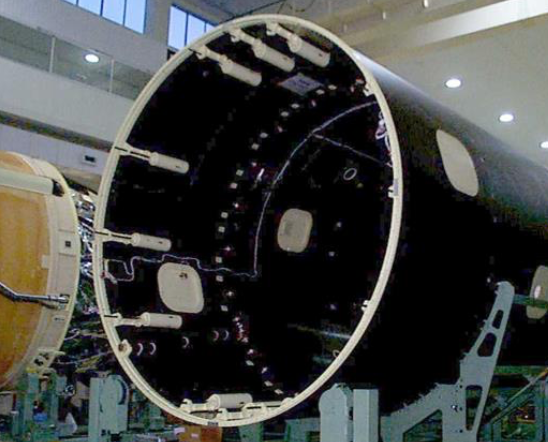
\includegraphics[width=\linewidth]{interstage_photo.png}\\
  {\scriptsize CFRP interstage structure of a launch vehicle.}
\end{column}
\end{columns}
\end{frame}

% ---------------------------------------------------------------------
\begin{frame}{Infrared stress measurement (DSPSS)}
\note{Our measurable quantity is infrared stress measurement. By the thermoelastic effect, a small temperature change is proportional to the change in the sum of principal stresses. So an infrared camera gives a full-field surface map of the stress sum, which we call DSPSS. A sub-surface defect perturbs this field and creates a local stress valley, as shown on the right.}
\begin{columns}[T]
\begin{column}{0.55\textwidth}
Thermoelastic effect relates a small temperature change to the change in
the sum of principal stresses:
\[
  \Delta T = -k\,T\,\Delta\sigma_{\mathrm{sum}},\qquad
  \sigma_{\mathrm{sum}} = \sigma_1+\sigma_2+\sigma_3 = \mathrm{tr}(\boldsymbol\sigma).
\]
Infrared stress measurement~\cite{ir1_main,ir1,sakagami2016} thus yields a
\textbf{full-field surface map} of $\sigma_{\mathrm{sum}}$ (DSPSS), from which
sub-surface defects are inferred.
\end{column}
\begin{column}{0.45\textwidth}
  \centering
  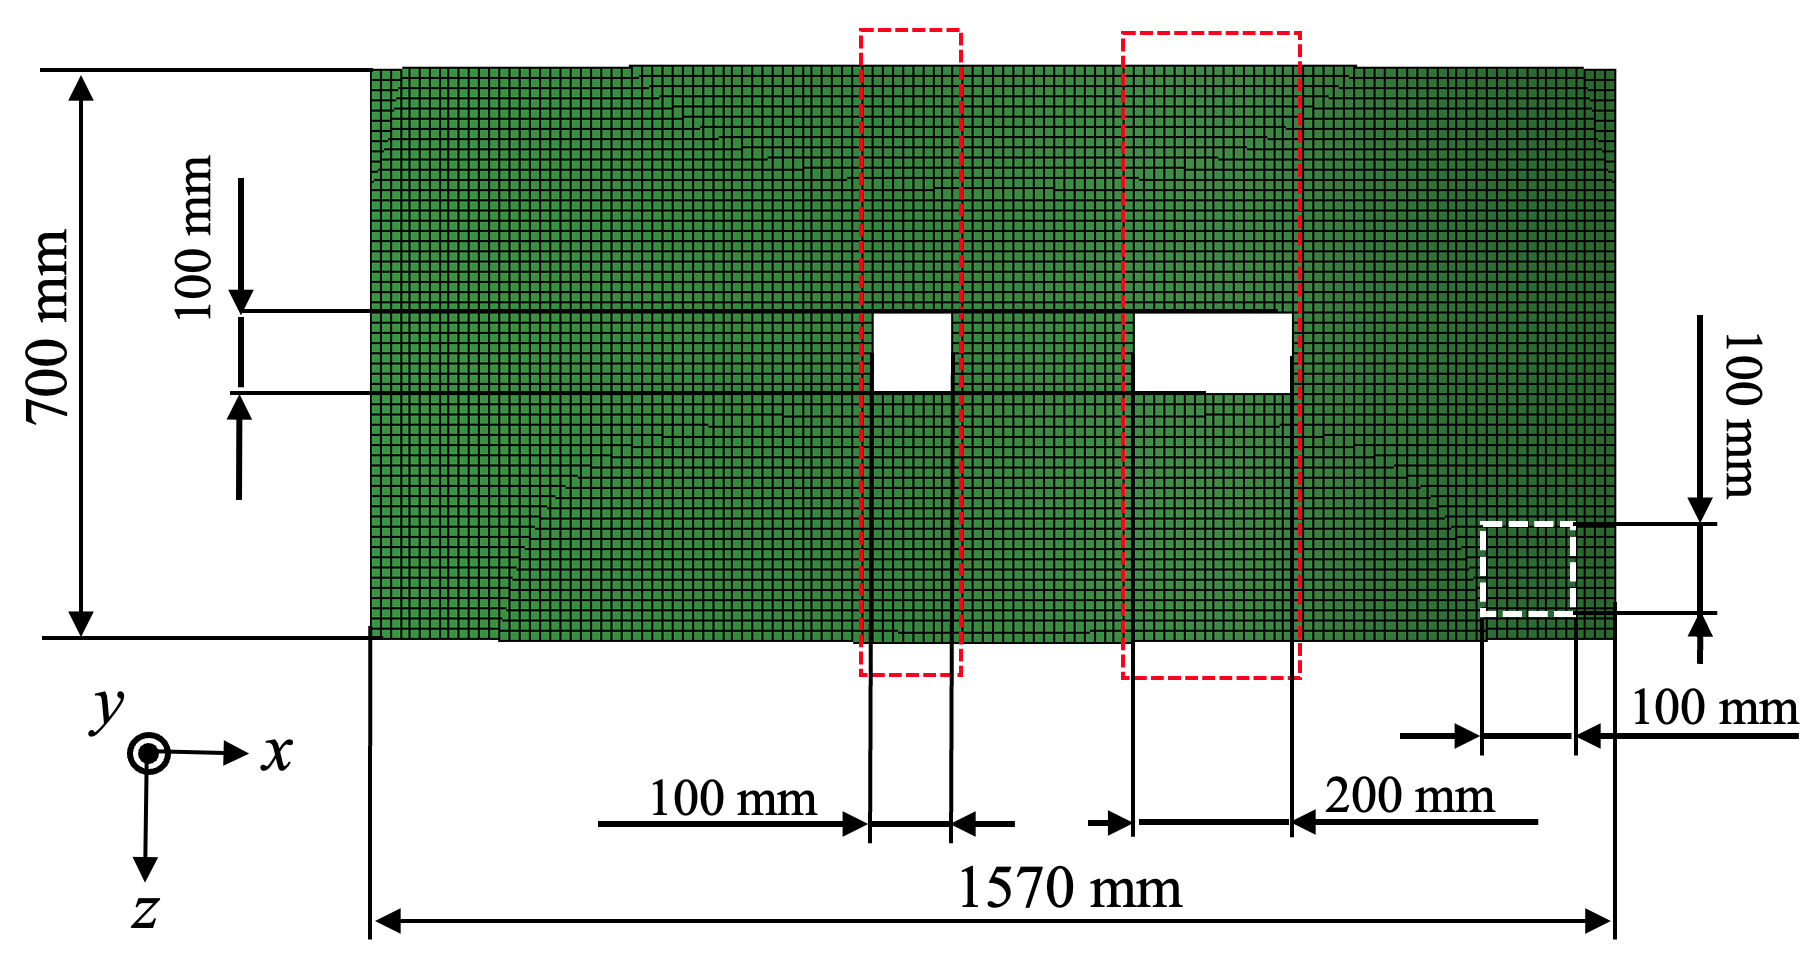
\includegraphics[width=\linewidth]{dspss_defect.png}\\
  {\scriptsize DSPSS shows a stress valley over the defect.}
\end{column}
\end{columns}
\end{frame}

% ---------------------------------------------------------------------
\begin{frame}{Previous study and purpose}
\note{Kojima et al. gave a CNN proof-of-concept on non-perforated CFRP. Our setting is harder: perforated interstage, full 3-D location (region times layer), and extreme imbalance. Formally we learn a node classifier on the mesh graph, minimizing focal loss; class zero is defect-free, classes one to eighteen encode region times layer.}
\begin{columns}[T]
\begin{column}{0.6\textwidth}
\textbf{Prior work.} Kojima \textit{et al.}~\cite{kojima,kojima2024_transfer} --- a CNN
\emph{proof-of-concept} on \emph{non-perforated} CFRP from FEM DSPSS.\\[2pt]
\textbf{This work --- harder setting:} \emph{perforated} interstage $\times$ \emph{3-D}
location (region $\times$ layer) $\times$ extreme imbalance ($<3\%$ defect nodes).
\end{column}
\begin{column}{0.4\textwidth}
  \centering
  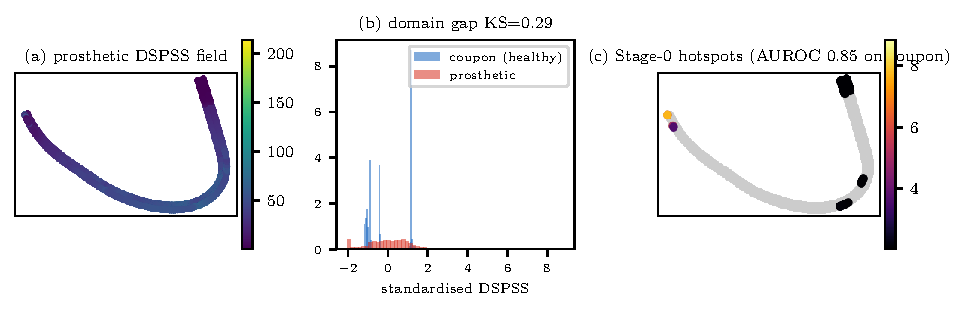
\includegraphics[width=\linewidth]{kojima_real.pdf}\\
  {\scriptsize Prior surface-stress lineage (Kojima \textit{et al.}).}
\end{column}
\end{columns}

\vspace{0.5em}
\textbf{Problem} --- node classification on the mesh graph $\mathcal G=(\mathcal V,\mathcal E)$,
node features $\mathbf x_i=(x,y,z,\hat\sigma_{\mathrm{sum}})_i$; learn
$f_\theta:\mathcal G\to\mathbb R^{|\mathcal V|\times 19}$,
\[
  \hat y_i=\!\arg\max_{c\in\{0,\dots,18\}}\!\big[\mathrm{softmax}\,f_\theta(\mathcal G)\big]_{i,c},
  \quad
  \theta^\star=\arg\min_{\theta}\sum_{i\in\mathcal V}\mathrm{FL}\!\big(p_{i,y_i}\big),
\]
class $0=$ defect-free; classes $1\text{–}18=$ (in-plane region $\times$ insertion layer).
\end{frame}

% ---------------------------------------------------------------------
\begin{frame}{Related work: where this work sits}
\note{Two anchors, both in Composites B. Kojima 2025 is the direct surface-stress lineage we build on (and a co-author). PIGMID 2026 is an adjacent physics-informed GNN, but on guided-wave sensor signals --- a different modality. We differentiate on input, structure, the physics prior, and the OOD generalization study.}
\footnotesize
\begin{tabular}{@{}lp{2.05cm}p{2.05cm}p{2.5cm}@{}}
\toprule
 & Kojima '25 (Compos.\ B) & PIGMID '26 (Compos.\ B) & \textbf{This work} \\
\midrule
Input    & surface stress (FEM$\to$IR) & guided waves (PZT$\times$8) & \textbf{full-field stress (DSPSS)} \\
Model    & transfer CNN & physics GNN (wave energy) & \textbf{mesh-physics GNN} \\
Geometry & simple coupons & instrumented plate & \textbf{perforated interstage, 3-D} \\
Physics  & noise-aug.\ sim pretrain & wave-energy adjacency & \textbf{FE-mesh topology $+$ DSPSS} \\
Novelty  & sim-to-real transfer & path heterogeneity & \textbf{OOD gen.\ $+$ detect/localize split} \\
\bottomrule
\end{tabular}
\vspace{0.6em}

{\small Unlike guided-wave GNNs (PIGMID) or simple-coupon transfer CNNs (Kojima~'25),
we learn on the structural FE mesh from full-field DSPSS, and are the first to
quantify OOD size/position generalization --- \textbf{detection transfers,
precise localization collapses}.}
\end{frame}

% ---------------------------------------------------------------------
\begin{frame}{FEM analysis conditions}
\note{We build the dataset by finite-element analysis: a one-eightieth-scale curved interstage panel, about 2 metres radius, with two rectangular holes. Delaminations are modeled explicitly by inserting thin Teflon sheets between selected plies, under tensile loading. This gives DSPSS fields with exactly known ground-truth defects.}
\begin{columns}[T]
\begin{column}{0.54\textwidth}
\begin{itemize}
  \item $1/80$-scale curved panel ($R\approx 2$\,m, $L\approx 1.57$\,m, $t=22$\,mm).
  \item Holes of $100\times100$ and $200\times100$\,mm.
  \item Sandwich laminate; tensile loading.
  \item Interlaminar delamination modeled explicitly by \textbf{Teflon inserts}
        between selected plies.
\end{itemize}
\vspace{0.3em}
\textbf{Dataset:} 1 reference $+$ \textbf{1386} defect specimens; 5-fold CV
($\approx$1110 train / 278 test per fold).
\end{column}
\begin{column}{0.46\textwidth}
  \centering
  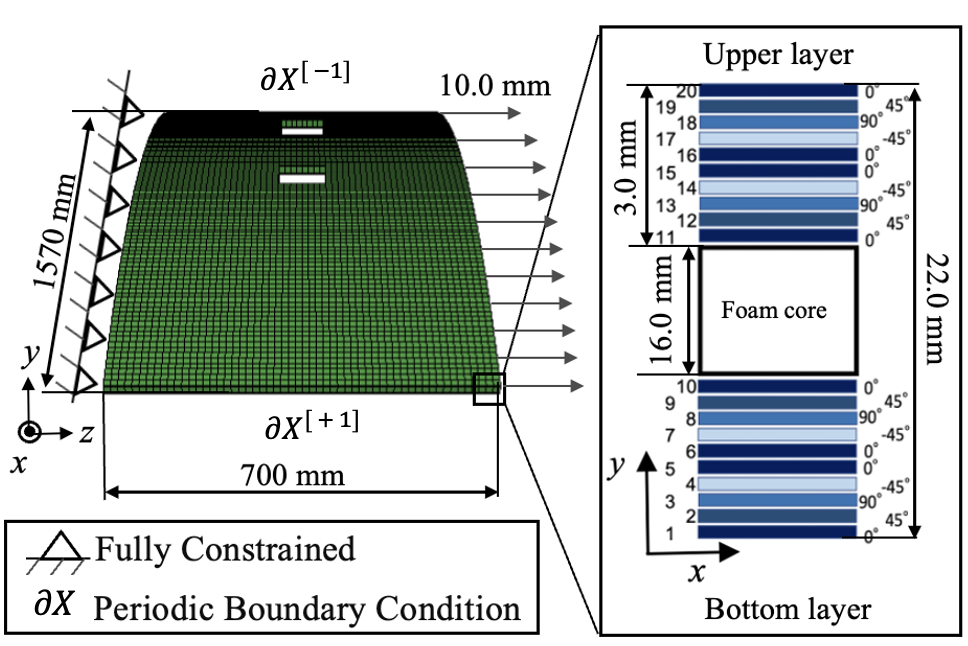
\includegraphics[width=\linewidth]{fem_condition.png}\\
  {\scriptsize FEM boundary conditions \& hole geometry.}
\end{column}
\end{columns}
\end{frame}

% ---------------------------------------------------------------------
\begin{frame}{Input data: normalized / difference DSPSS}
\note{The raw DSPSS is dominated by the stress concentration around the holes, which masks the defect. So we subtract a defect-free reference to get a difference field, and z-score normalize per node. This isolates the defect signal and, importantly, improves discrimination in the depth direction --- that is, which layer the defect is in.}
\begin{columns}[T]
\begin{column}{0.52\textwidth}
Raw DSPSS is dominated by \textbf{stress concentration around the hole},
masking the defect signal.

\vspace{0.5em}
Remedy (paper):
\begin{itemize}
  \item \textbf{Difference} field: damaged $-$ defect-free reference;
  \item \textbf{Z-score normalization} (per node), improving depth discrimination.
\end{itemize}
\vspace{-0.2em}
\[
  d_i=\sigma_i^{\mathrm{dmg}}-\sigma_i^{\mathrm{ref}},\qquad
  \hat\sigma_i=\frac{d_i-\mu_d}{s_d}.
\]
$\Rightarrow$ robust localization even near the opening.
\end{column}
\begin{column}{0.48\textwidth}
  \centering
  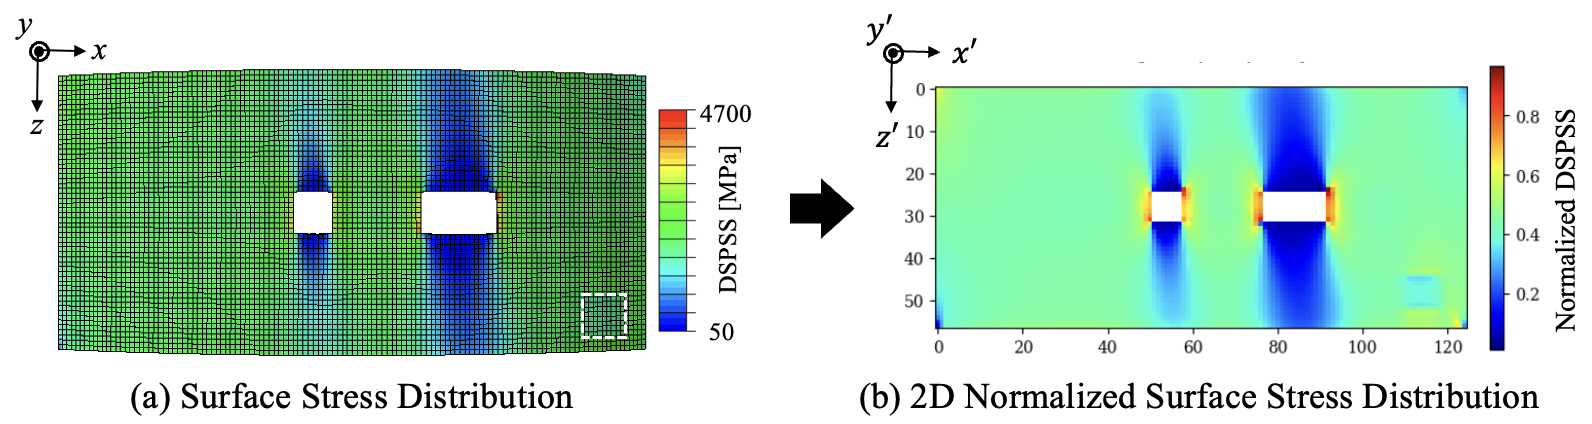
\includegraphics[width=\linewidth]{dspss_normalized.png}\\
  {\scriptsize Normalized DSPSS isolates the defect.}
\end{column}
\end{columns}
\end{frame}

% ---------------------------------------------------------------------
\begin{frame}{Stress distribution around the defect}
\note{Looking closer, each defect produces a stress valley at its centre. The depth and width of that valley depend on the ply angle above it: ninety-degree plies give sharp narrow valleys, zero and forty-five broaden them. This ply-angle signature is exactly the cue the network uses to tell which layer the delamination is in. It is a fine spatial-frequency problem, which motivates local attention.}
\begin{columns}[T]
\begin{column}{0.54\textwidth}
\begin{itemize}
  \item DSPSS exhibits a clear \textbf{stress valley} at the defect centre.
  \item Depth and width of the valley depend on \textbf{ply angle}:
        $90^\circ$ plies give sharp narrow valleys; $0^\circ/45^\circ$ broaden them.
  \item This signature tells the network \emph{which layer} the delamination sits in.
\end{itemize}
\vspace{0.3em}
\begin{exampleblock}{Implication}
Layer discrimination is a \emph{fine spatial-frequency} problem — motivating
local attention.
\end{exampleblock}
\end{column}
\begin{column}{0.46\textwidth}
  \centering
  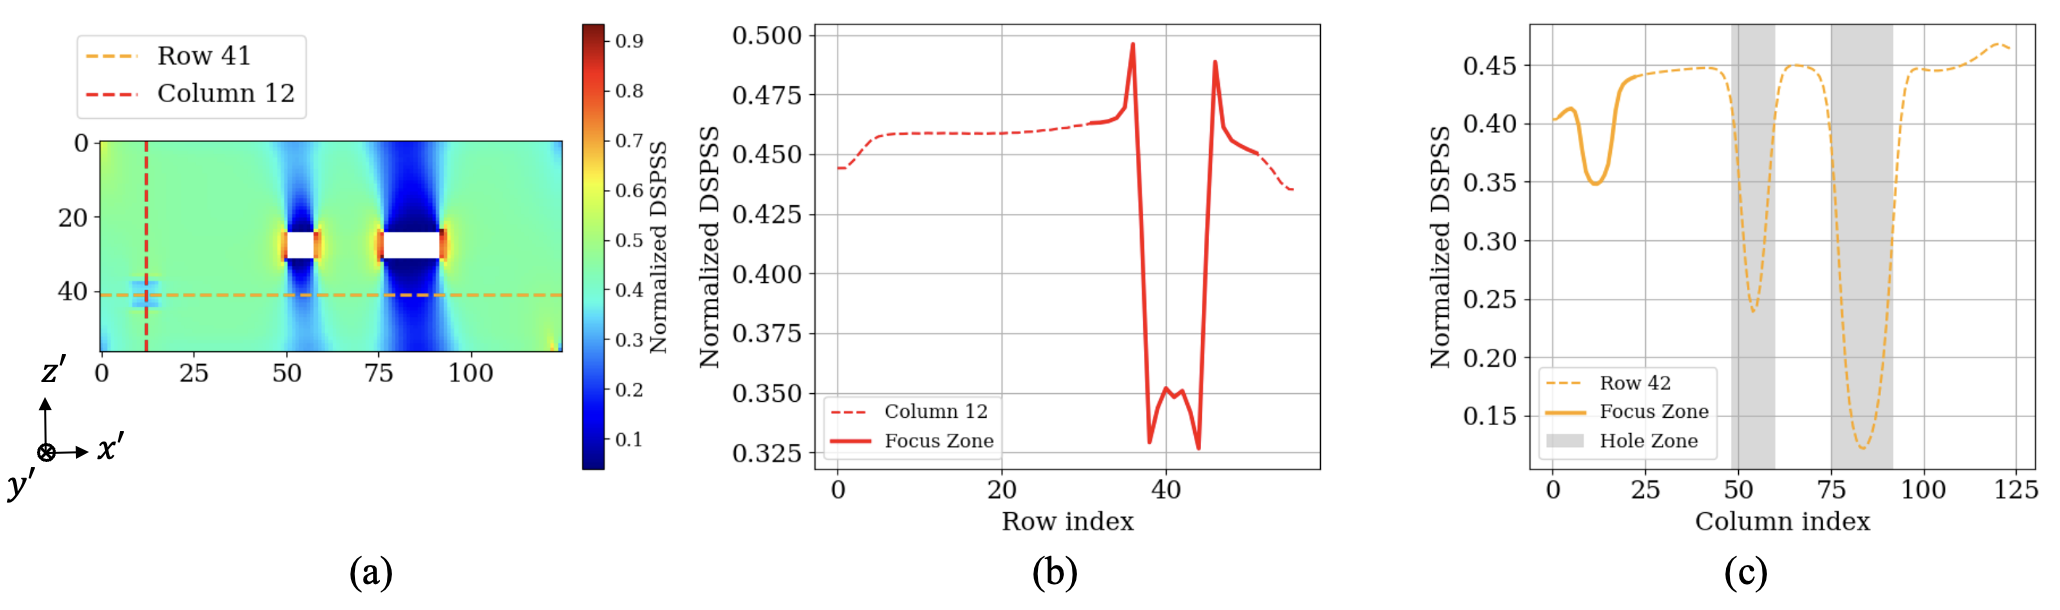
\includegraphics[width=\linewidth]{dspss_profile.png}\\
  {\scriptsize Normalized DSPSS profile across the defect.}
\end{column}
\end{columns}
\end{frame}

% ---------------------------------------------------------------------
\begin{frame}{Detect first, then localize --- screening comes for free}
\note{One quick but important point before the network. Detection and localization are different jobs. Detection --- is there a defect, and roughly where --- needs no learning at all. Because every specimen shares one mesh geometry, the healthy fields form a point cloud around a single template, so the same per-node z-score we already use as input doubles as an unsupervised detector: score each node by how many standard deviations it sits from the healthy mean, with mean and std estimated from two thousand defect-free fields. On clean data this per-node statistic reaches node-level AUROC of about one --- it actually beats every learned anomaly detector we tried, including a diffusion model. The one caveat is signal-to-noise, but it is more forgiving than folklore suggests: on a labelled coupon the detector still scores about 0.84 AUROC at noise one-tenth of the field standard deviation, and only falls to chance near seven-tenths to one times the field std --- so the often-quoted collapse at sigma equals 0.1 is wrong. Lock-in infrared thermography, where noise falls as one over root-K frames, only adds margin. So screening is cheap. The GNN earns its keep on the genuinely hard part: the semantic nineteen-class region-by-layer identification under noise --- which is the rest of this talk.}
\begin{columns}[T]
\begin{column}{0.5\textwidth}
\textbf{Two different jobs.} \emph{Detection} (is there / where?) needs
\textbf{no learning}: every specimen shares one mesh, so healthy fields are a
point cloud around \emph{one} template.

\vspace{0.5em}
The \emph{same} per-node z-score we feed the GNN doubles as an unsupervised
screen:
\[
  s_i = \frac{|x_i-\mu_i|}{\sigma_i},\qquad
  (\mu_i,\sigma_i)\ \text{from } N{=}2000\ \text{healthy fields.}
\]
Node-level, label-free, $\sim$30 lines, CPU-minutes.
\end{column}
\begin{column}{0.5\textwidth}
\begin{block}{Node AUROC (clean)}
\best{Per-node Mahalanobis / PCA: $0.999\,/\,0.995$} (2$\times$2 / 4$\times$4).\\[2pt]
{\scriptsize Learned baselines: PaDiM $0.96$, PatchCore $0.93$,
STFPM $0.75$, diffusion $0.50$--$0.66$.}
\end{block}
\begin{alertblock}{SNR: robust, not fragile}
Verified on a labelled coupon: detection holds (AUROC ${\sim}0.84$) at noise
$\sigma{=}0.1$ of field std, failing only near $\sigma{\approx}0.7$--$1.0$ ---
not the folklore ``$0.1$ collapse.'' Lock-in IR ($\sigma\!\propto\!1/\sqrt{K}$)
adds margin.
\end{alertblock}
\end{column}
\end{columns}
\vspace{0.3em}
$\Rightarrow$ detection is cheap; the GNN is for the hard part ---
\textbf{semantic 19-class (region $\times$ layer) localization} under noise.
\end{frame}

% ---------------------------------------------------------------------
\begin{frame}{Graph representation \& GAT model}
\note{We represent each surface element as a node, with features being its coordinates and the normalized stress. Edges are the fixed mesh connectivity, reused across all specimens. We use a graph attention network: three GAT layers, sixty-four to two-hundred-fifty-six channels, multi-head, with batch-norm, dropout and residual connections. Attention lets each node weight its neighbours adaptively, which suits the highly non-uniform stress field.}
\begin{columns}[T]
\begin{column}{0.5\textwidth}
Nodes $=$ elements ($\mathbf x_i$), edges $=$ fixed mesh connectivity.
GAT message passing~\cite{gat1,gnn1,gilmer2017mpnn}:
\vspace{-0.3em}
\[
  e_{ij}=\mathrm{LeakyReLU}\!\big(\mathbf a^{\!\top}[\mathbf W\mathbf h_i\,\Vert\,\mathbf W\mathbf h_j]\big),
\]
\vspace{-0.9em}
\[
  \alpha_{ij}=\frac{\exp e_{ij}}{\sum_{k\in\mathcal N(i)}\exp e_{ik}},
\]
\vspace{-0.9em}
\[
  \mathbf h_i'=\Big\Vert_{m=1}^{M}\,\sigma\!\Big(\sum_{j\in\mathcal N(i)}\alpha_{ij}^{(m)}\mathbf W^{(m)}\mathbf h_j\Big).
\]
{\scriptsize $3$ layers $64\!\to\!256\!\to\!256$, $M$ heads, BN $+$ dropout $+$ residual.}
\end{column}
\begin{column}{0.5\textwidth}
  \centering
  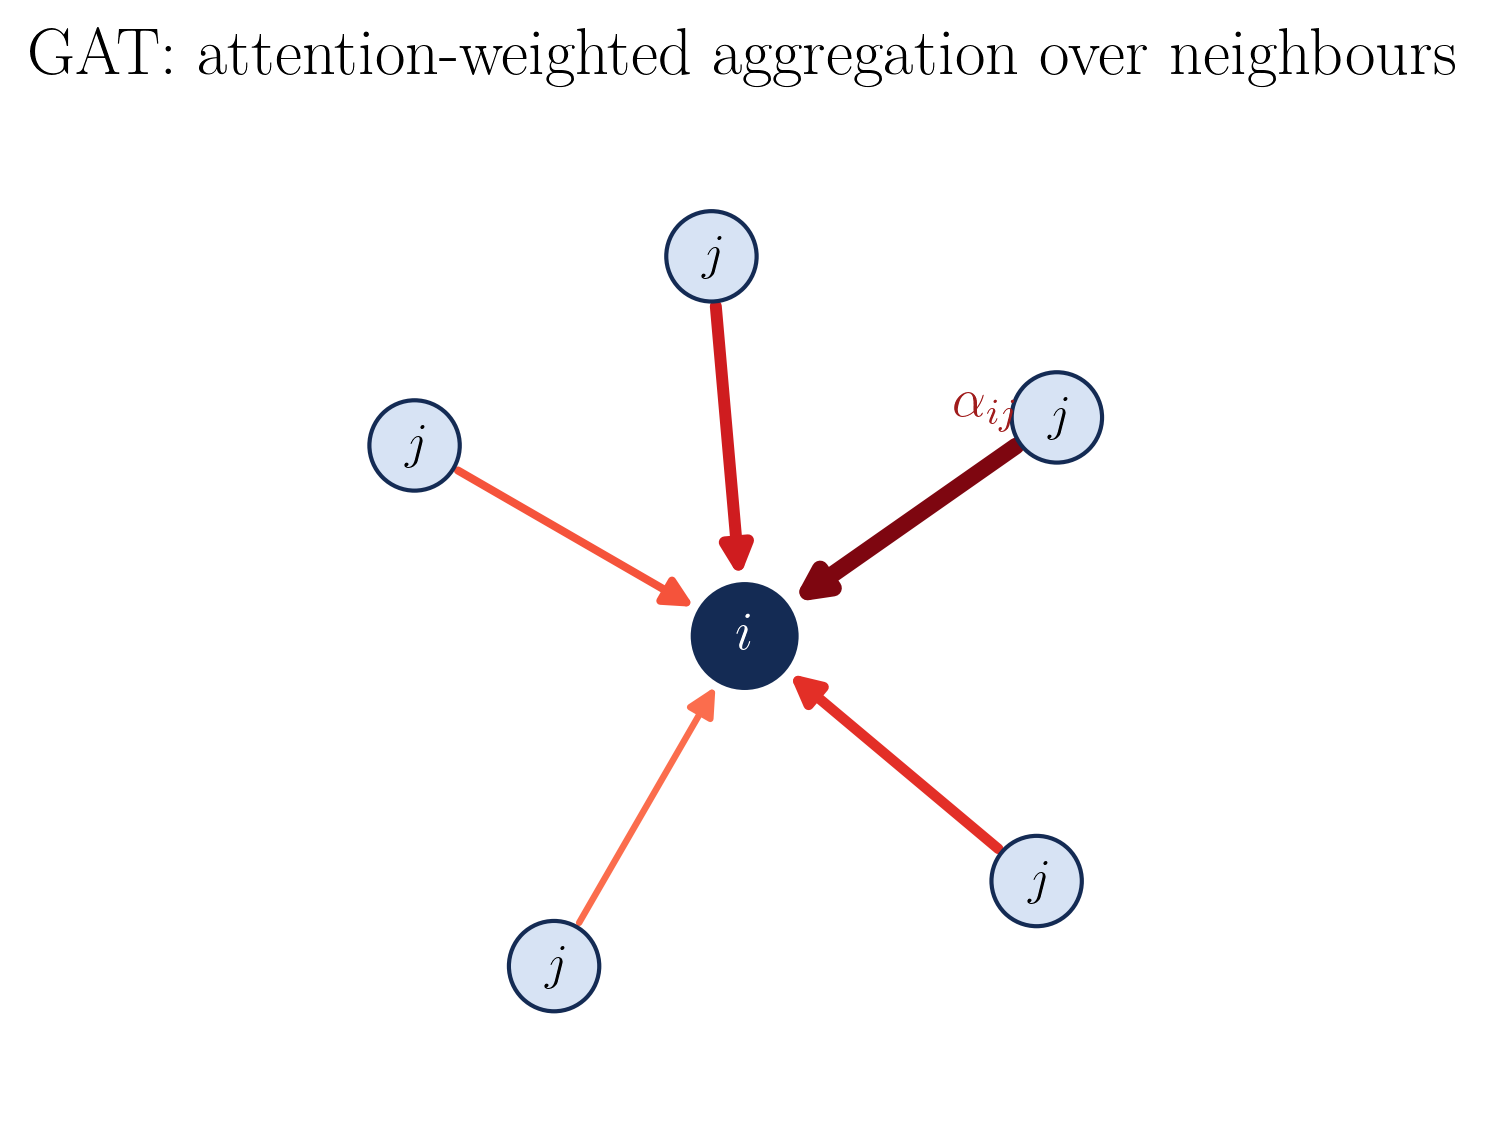
\includegraphics[width=0.92\linewidth]{gat_attention.png}\\
  {\scriptsize Attention-weighted aggregation; arrow thickness $\propto \alpha_{ij}$.}
\end{column}
\end{columns}
\end{frame}

% ---------------------------------------------------------------------
\begin{frame}{Output: 3-D defect location as 19-class node labels}
\note{We formulate localization as node classification into nineteen classes: class zero is defect-free, and the other classes jointly encode the in-plane region and the insertion layer. We label only one side, so prediction needs a single surface measurement. Note the severe imbalance --- defect nodes are under three percent of all nodes.}
\begin{columns}[T]
\begin{column}{0.52\textwidth}
\begin{itemize}
  \item Node classification into \textbf{19 classes}:
        class 0 $=$ defect-free; remaining classes encode
        \emph{in-plane region} $\times$ \emph{insertion layer}.
  \item One-side labelling so prediction needs only single-surface DSPSS.
\end{itemize}
\[
  p_{i,c}=\frac{e^{z_{i,c}}}{\sum_{k=0}^{18} e^{z_{i,k}}},\qquad
  \hat y_i=\arg\max_{c} \,p_{i,c}.
\]
\begin{block}{Severe imbalance}
Defect nodes are $<3\%$ of all nodes — handled by the loss (next slide).
\end{block}
\end{column}
\begin{column}{0.48\textwidth}
  \centering
  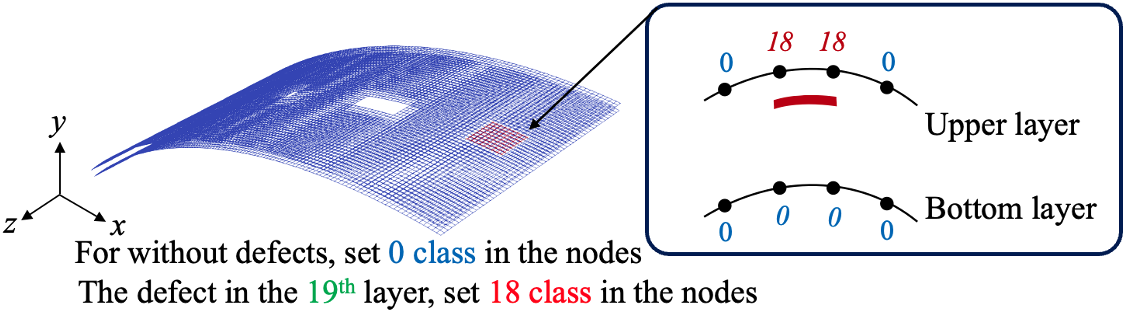
\includegraphics[width=\linewidth]{label19.png}\\
  {\scriptsize 19-class label map.}
\end{column}
\end{columns}
\end{frame}

% ---------------------------------------------------------------------
\begin{frame}{Loss function: Focal loss}
\note{To handle that imbalance we use focal loss, which down-weights the easy, abundant defect-free nodes and focuses learning on the rare defect classes. Without it, the model simply predicts defect-free everywhere.}
\begin{columns}[T]
\begin{column}{0.52\textwidth}
\[
  \mathrm{FL}(p_t) = -\,\alpha_t\,(1-p_t)^{\gamma}\,\log p_t .
\]
\begin{itemize}
  \item Down-weights easy, abundant defect-free nodes;
        emphasises rare defect-class nodes~\cite{focal_loss}.
  \item Crucial because intact regions dominate ($>97\%$).
\end{itemize}
\end{column}
\begin{column}{0.48\textwidth}
  \centering
  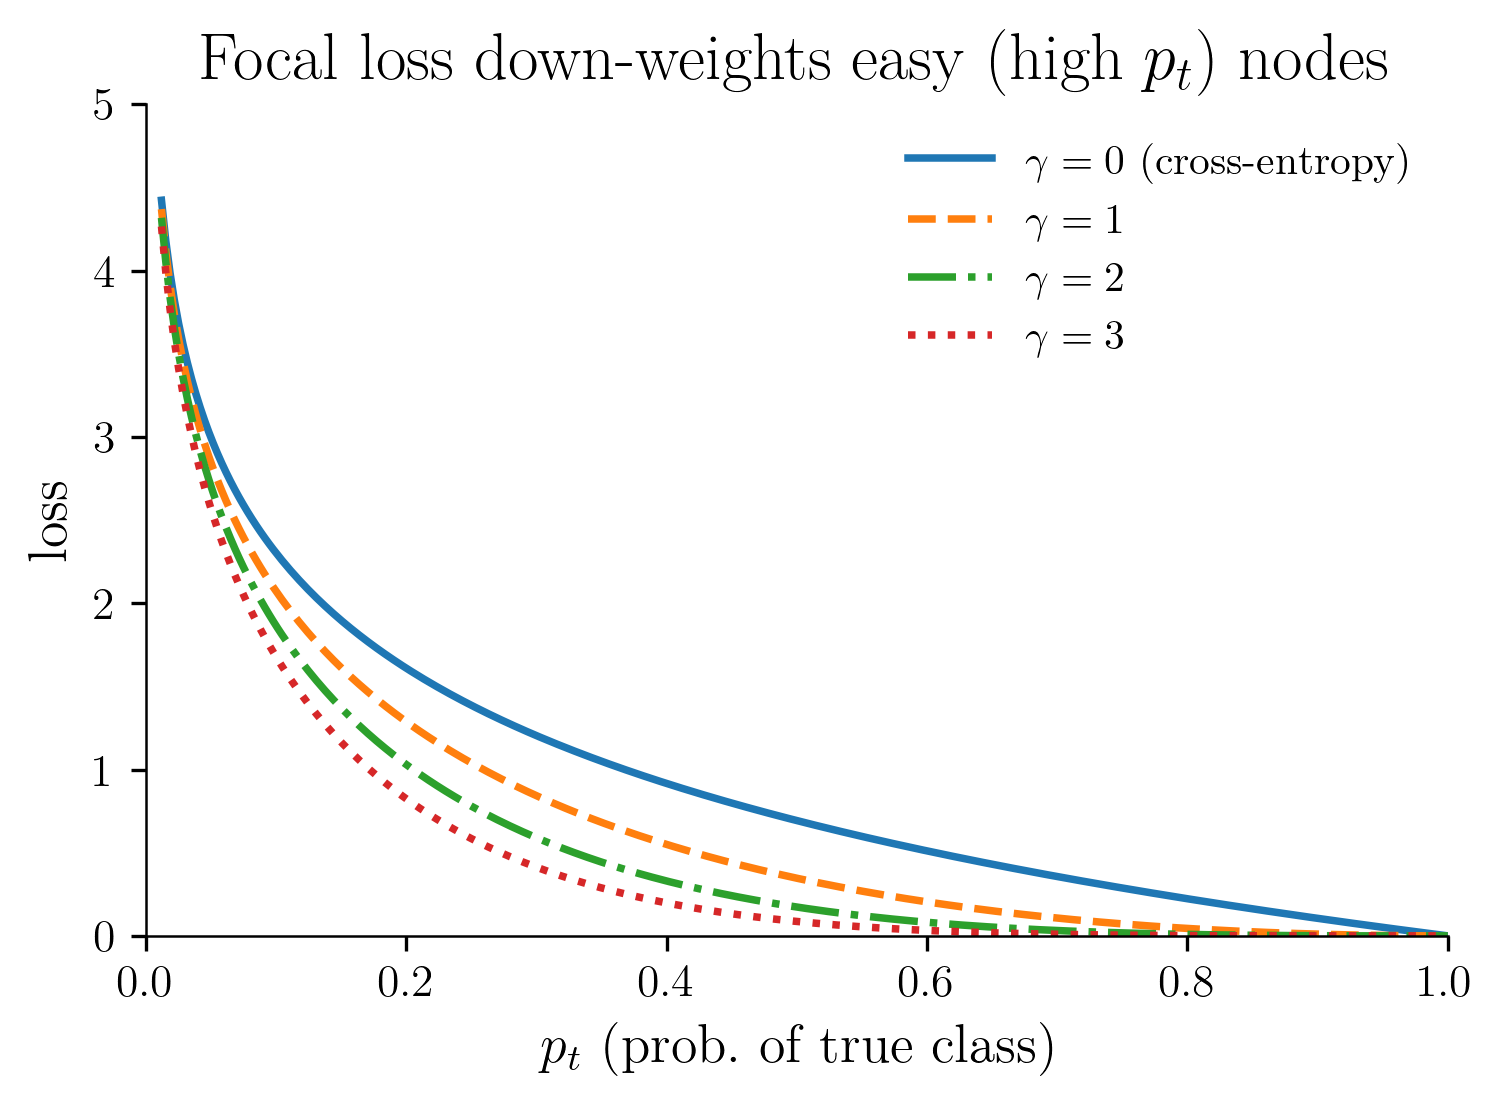
\includegraphics[width=\linewidth]{focal_curve.png}
\end{column}
\end{columns}
\end{frame}

% ---------------------------------------------------------------------
\begin{frame}{Results: prediction accuracy}
\note{On held-out test specimens we get a planar score R of 0.72, a depth score of 0.69, and a combined TDPS of 0.70, up to 0.92 in the best case. The mid-thickness layers, nine to twelve, are localized best. Critically, the false-negative rate on defect nodes is under three percent, so we rarely miss a real defect.}
\begin{columns}[T]
\begin{column}{0.5\textwidth}
Test-set metrics:
\begin{itemize}
  \item planar $R = 0.72$ (mean), depth $P_{\mathrm{gauss}} = 0.69$,
        combined $\mathrm{TDPS} = 0.70$ (best $0.92$).
  \item Best layers: 9--12 (mid-thickness); Layer-10 samples all
        $\mathrm{TDPS}\ge 0.82$.
  \item False-negative rate for defect nodes \textbf{$<3\%$}.
\end{itemize}
\vspace{0.3em}
{\scriptsize $R$: planar F1.\quad $P_{\mathrm{gauss}}$: Gaussian depth score ($\sigma{=}2$).\quad
$\mathrm{TDPS}=\tfrac12(R{+}P_{\mathrm{gauss}})$.}
\end{column}
\begin{column}{0.5\textwidth}
  \centering
  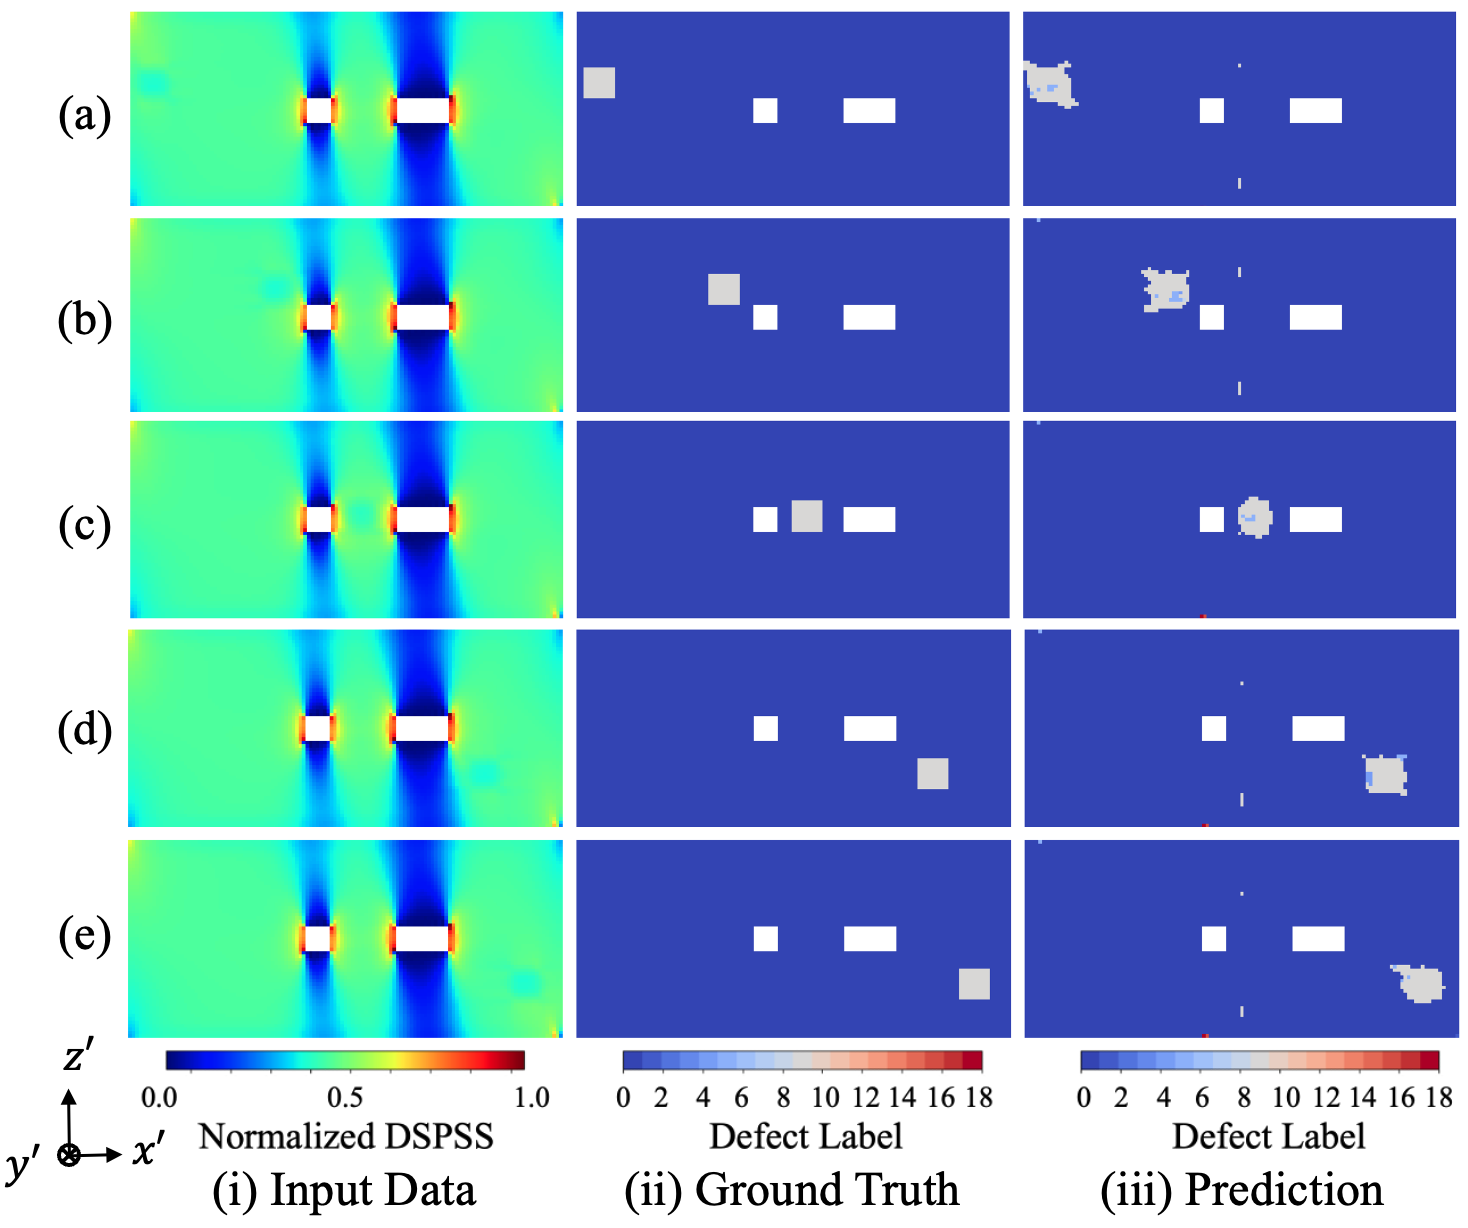
\includegraphics[width=\linewidth]{pred_l10.png}\\
  {\scriptsize Input $\rightarrow$ ground truth $\rightarrow$ prediction (Layer-10 cases).}
\end{column}
\end{columns}
\end{frame}

% ---------------------------------------------------------------------
\begin{frame}{Overall performance \& confusion}
\note{Overall macro-F1 is sixty-one percent across all nineteen classes, from surface DSPSS alone. The confusion matrix has a strong diagonal; the residual errors are mostly confusion with the adjacent layer, and false positives cluster near the hole edge, where stress gradients are steep.}
\begin{columns}[T]
\begin{column}{0.5\textwidth}
  \begin{block}{Headline}
  \best{Macro-F1 $= 61\%$} across 19 classes, using \emph{surface DSPSS only}.
  \end{block}
  \[
    \mathrm{F1}_c=\frac{2P_cR_c}{P_c+R_c},\quad
    \text{macro-F1}=\frac{1}{19}\sum_{c=0}^{18}\mathrm{F1}_c.
  \]
  \begin{itemize}
    \item Dominant diagonal; residual \emph{adjacent-layer} confusion.
    \item False positives cluster near the hole edge.
    \item Robust across defect insertion regions.
  \end{itemize}
\end{column}
\begin{column}{0.5\textwidth}
  \centering
  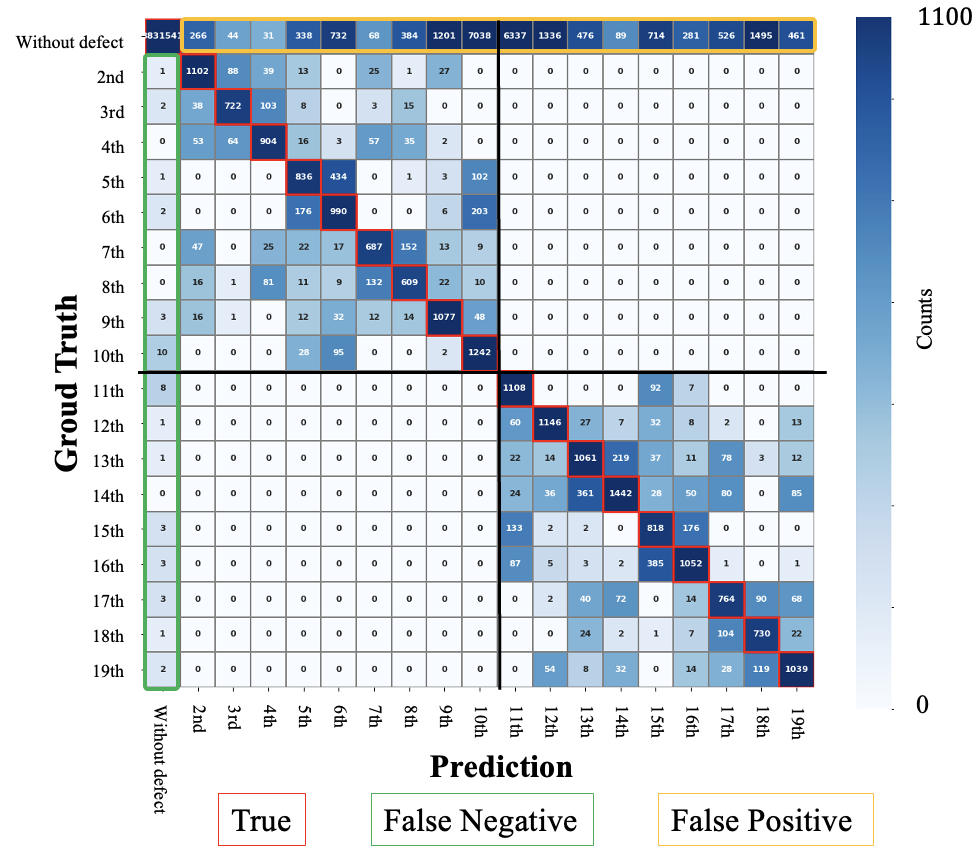
\includegraphics[width=\linewidth]{confusion_61.png}\\
  {\scriptsize Confusion matrix (macro-F1 61\%).}
\end{column}
\end{columns}
\end{frame}

% ---------------------------------------------------------------------
\begin{frame}{Conclusion}
\note{To summarize the published work: an FEM-plus-GAT framework localizes 3-D delamination in perforated CFRP; difference-normalized DSPSS removes the hole concentration and enables full-region estimation; and we reach sixty-one percent macro-F1 from surface data alone, with very low false negatives and no false detections in healthy regions.}
\begin{itemize}
  \item Introduced an \textbf{FEM + GAT} framework for 3-D delamination
        localization in perforated CFRP interstage panels.
  \item \textbf{Difference-normalized DSPSS} suppresses hole stress
        concentration and enables full-region estimation.
  \item Achieved \best{macro-F1 $61\%$} on 19 classes from surface data only,
        with a very low defect false-negative rate and no false detections in
        defect-free regions.
\end{itemize}
\vspace{0.3em}
\begin{block}{A scalable foundation}
toward experimental infrared-stress (TSA) data and practical SHM of aerospace
composite structures.
\end{block}
\end{frame}

% =====================================================================
%  NEW CONTRIBUTION (beyond last year's paper): noise robustness + NDF.
%  This is exactly the WCCM-abstract delta ("robustness under
%  experimentally motivated noise conditions") — co-author-vetted.
% =====================================================================
\begin{frame}{New focus: robustness for real operation}
\note{Now the new part for this congress. The published model assumes clean FEM fields. Real infrared measurements carry noise --- temperature drift, emissivity, sensor noise. And in practice almost the entire structure is healthy, so false alarms are very costly. So here we focus on robustness under realistic noise and on suppressing false detection. On the right, the input with and without injected noise --- the defect signature still survives.}
\begin{columns}[T]
\begin{column}{0.52\textwidth}
The published model assumes clean FEM fields. In practice infrared measurement
carries \textbf{acquisition noise}, and almost the whole structure is
\textbf{defect-free} — false alarms are costly.
\end{column}
\begin{column}{0.48\textwidth}
\begin{alertblock}{WCCM contribution}
Robustness under realistic noise \emph{and} explicit suppression of false
detection on healthy regions.
\end{alertblock}
\end{column}
\end{columns}
\vspace{0.4em}
\begin{center}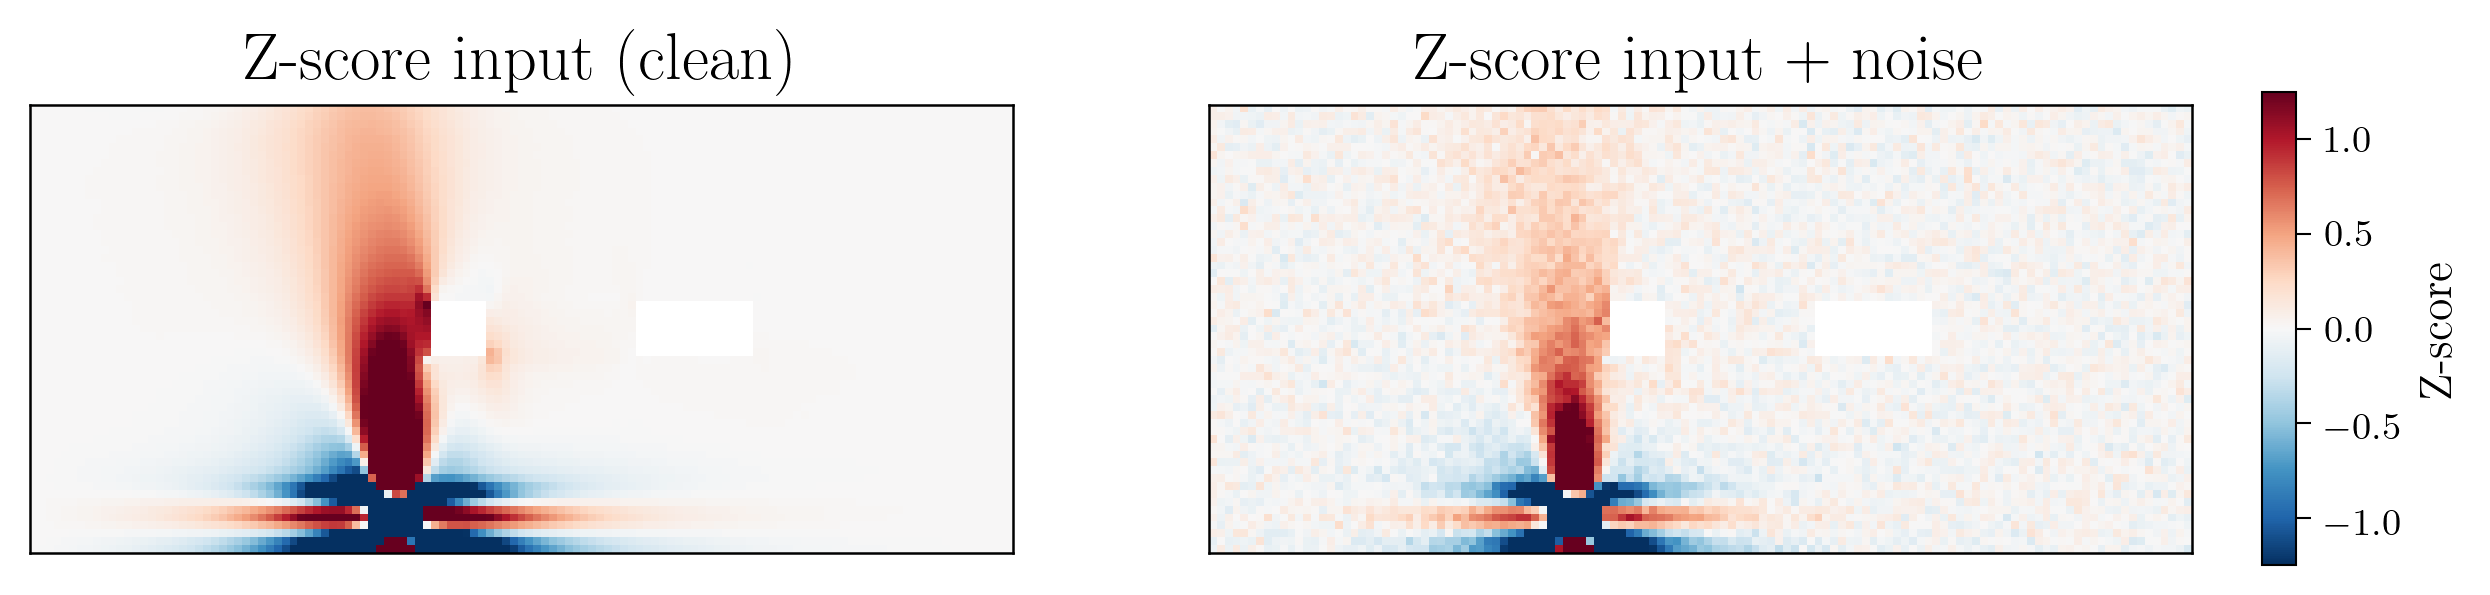
\includegraphics[width=0.92\linewidth]{noise_clean.png}\end{center}
\vspace{-0.4em}{\centering\scriptsize Clean vs.\ noise-injected Z-score input — the defect signature survives.\par}
\end{frame}

% ---------------------------------------------------------------------
\begin{frame}{Noise-augmented dataset \& defect-free negatives (NDF)}
\note{We do two things. First, defect-free negatives: we add five thousand samples that are a zero field plus Gaussian noise at ten percent of the data standard deviation, so the model explicitly learns what no-defect looks like. Second, we add structured noise to the defect data --- line noise along the fibre direction, attenuated noise across it, and global white noise --- to mimic measurement artefacts.}
\begin{columns}[T]
\begin{column}{0.5\textwidth}
\textbf{Defect-free negatives (NDF):} zero field $+$ Gaussian noise
($10\%$ of data std), $5{,}000$ samples added to training.
\end{column}
\begin{column}{0.5\textwidth}
\textbf{Structured noise on defect data:} line noise along the fibre ($z$),
attenuated noise in $x$, and global white noise.
\end{column}
\end{columns}
\vspace{0.4em}
\begin{center}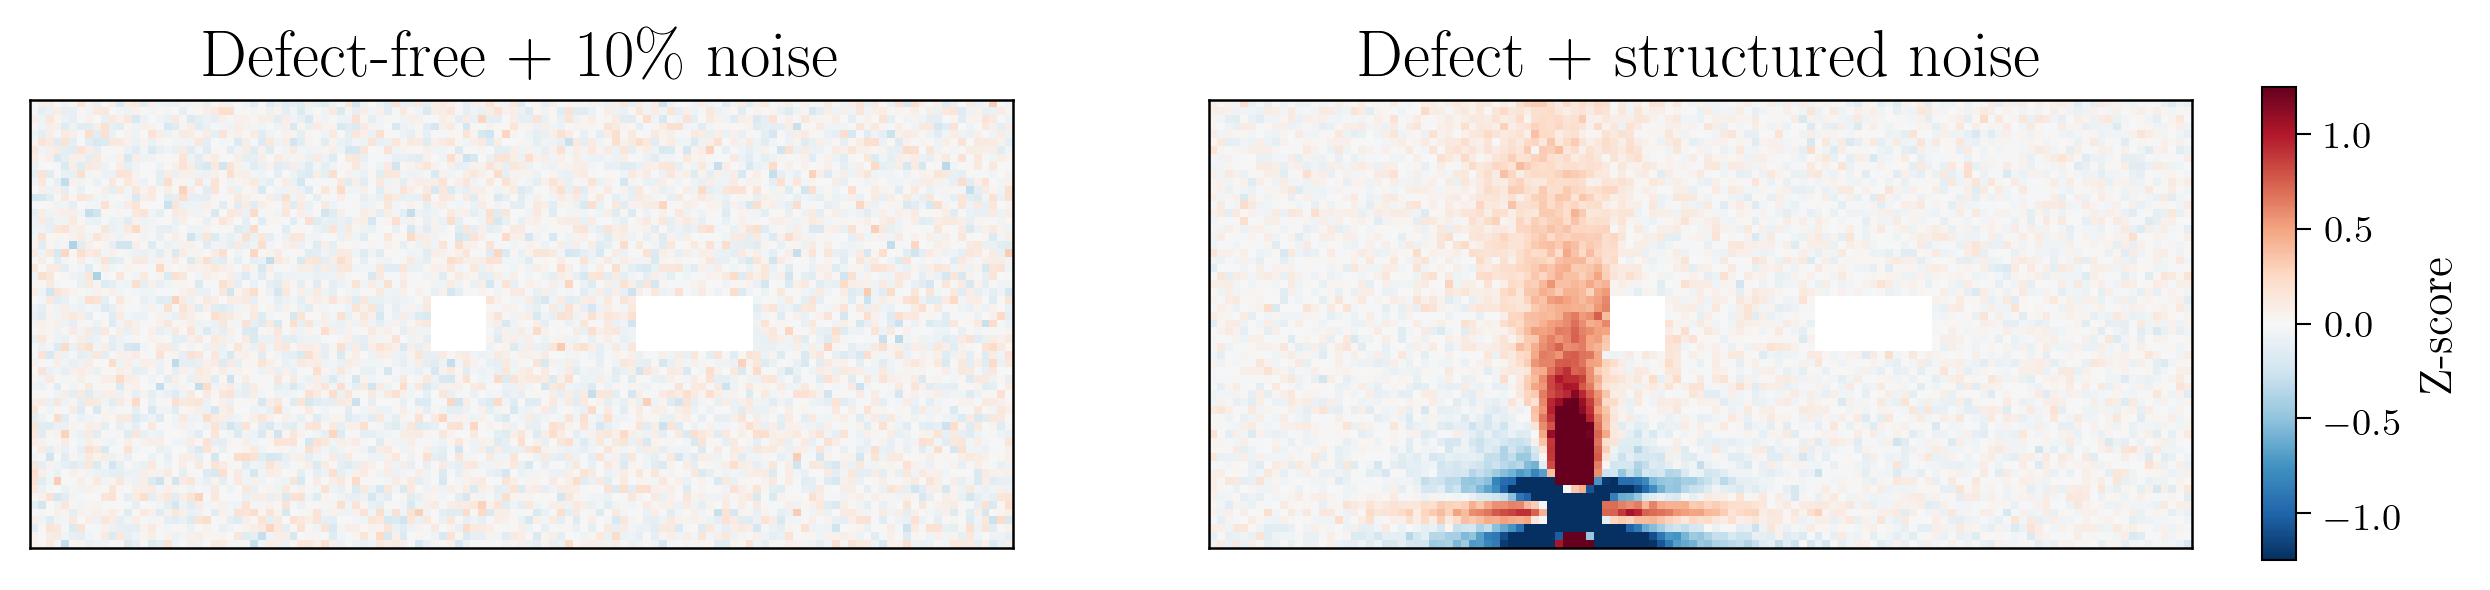
\includegraphics[width=0.92\linewidth]{ndf2_clean.png}\end{center}
\vspace{-0.4em}{\centering\scriptsize Left: defect-free $+$ noise (teaches ``no defect''). \ Right: defect $+$ structured noise.\par}
\end{frame}

% ---------------------------------------------------------------------
\begin{frame}{Results under noise}
\note{The outcome: with the difference-DSPSS input, the model still estimates defects across the full region; prediction stays accurate on noise-injected data; and the defect-free negatives remove spurious activations, so we get essentially no false detection on healthy inputs. Here, the noisy input on the left still yields the correct target localization on the right. This makes the framework robust enough to move toward real experimental data.}
\begin{itemize}
  \item Difference-DSPSS input enables \textbf{full-region} defect estimation;
        prediction stays accurate on \textbf{noise-injected} data.
  \item \textbf{No false detection} on defect-free inputs — the NDF negatives
        remove spurious activations. $\Rightarrow$ robust enough to move toward
        \emph{experimental} infrared stress data.
\end{itemize}
\vspace{0.2em}
\begin{center}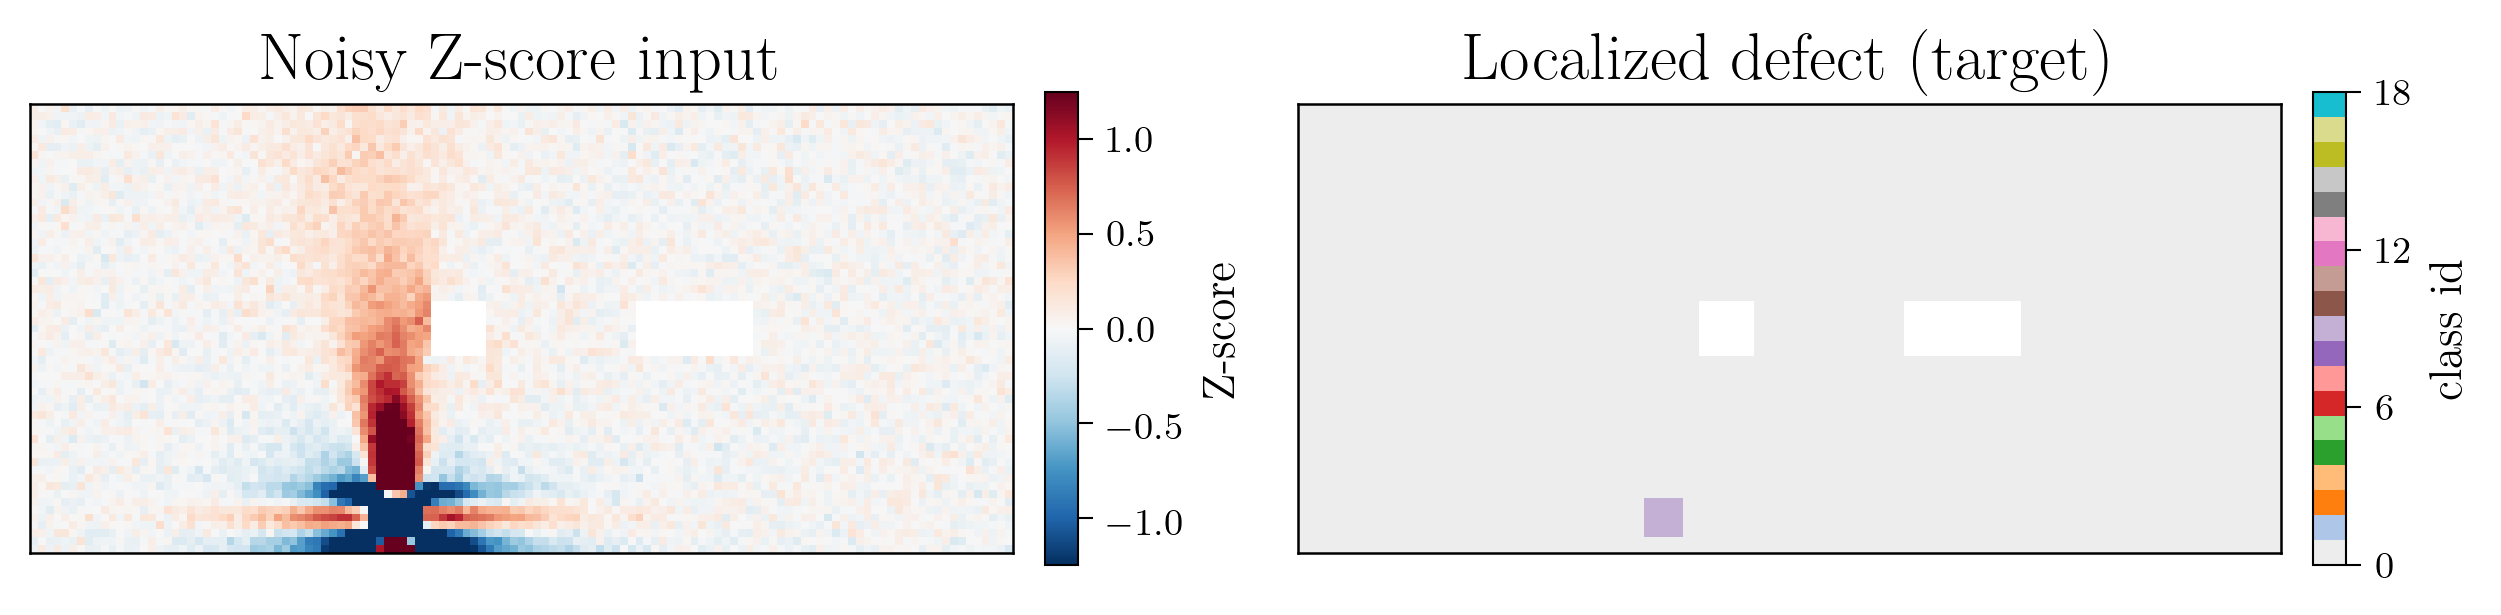
\includegraphics[width=0.92\linewidth]{result_clean.png}\end{center}
\vspace{-0.4em}{\centering\scriptsize Noisy input (left) $\rightarrow$ correct defect localization (right).\par}
\end{frame}

% ---------------------------------------------------------------------
\begin{frame}{Outlook \quad {\small[ongoing, beyond the published paper]}}
\note{Going forward: first, sim-to-real --- applying this noise-robust model to actual infrared stress measurements. Second, and still preliminary, we are extending from attention GNNs to mesh-physics GNNs such as MeshGraphNet and some layered variants; early results are encouraging and under evaluation with our co-authors. And third, transferring the approach to payload-fairing structural health monitoring. I will stop here. Thank you --- I am happy to take questions.}
\small
\begin{itemize}\itemsep2pt
  \item \textbf{Sim-to-real:} apply the noise-robust model to \emph{experimental}
        infrared-stress (TSA) measurements.
  \item \textbf{Architecture study (preliminary):} extending from attention
        GNNs to \emph{mesh-physics} GNNs (MeshGraphNet) and layered variants;
        early results are encouraging and under evaluation with co-authors.
  \item \textbf{Application:} transfer to other perforated / bonded CFRP structures ---
        rocket motor cases, aircraft wing boxes, satellite panels, payload-fairing SHM.
\end{itemize}
\vspace{0.2em}
\begin{columns}[T]
\begin{column}{0.32\textwidth}\centering
  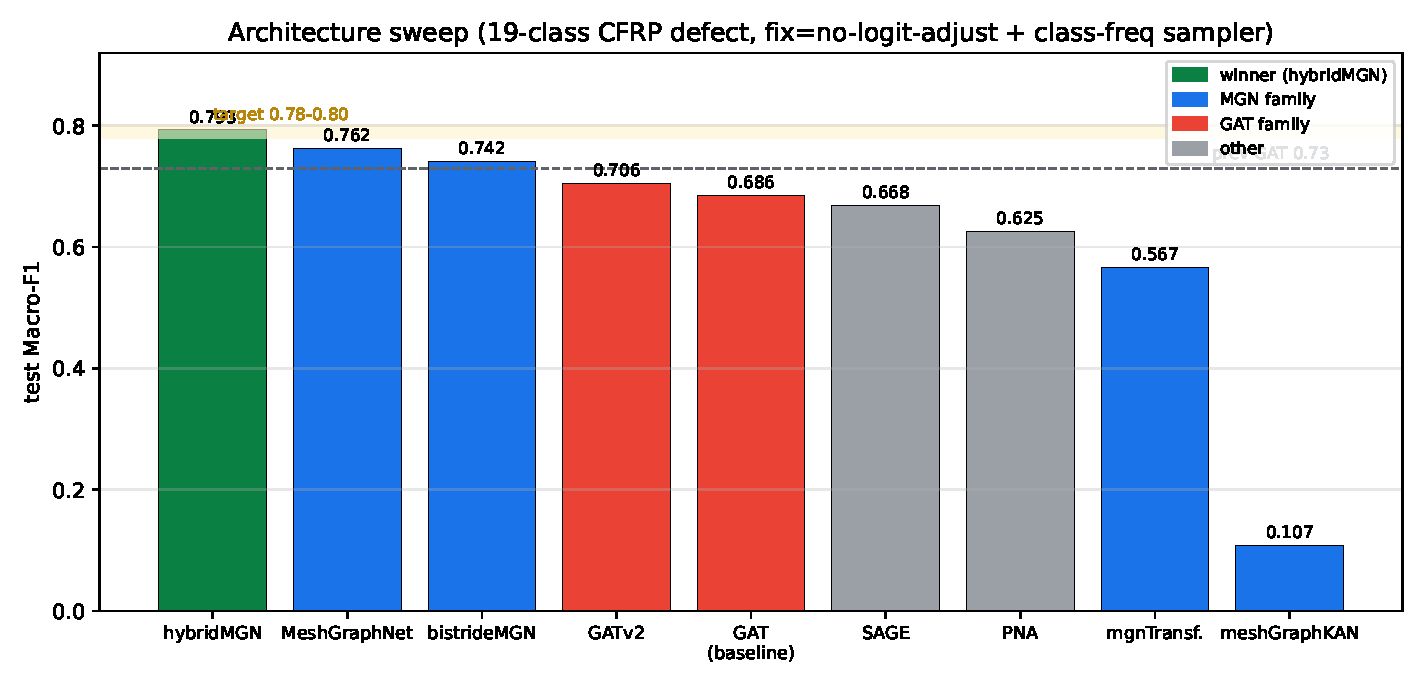
\includegraphics[height=2.2cm]{arch_sweep.pdf}\\{\scriptsize Architecture study}
\end{column}
\begin{column}{0.32\textwidth}\centering
  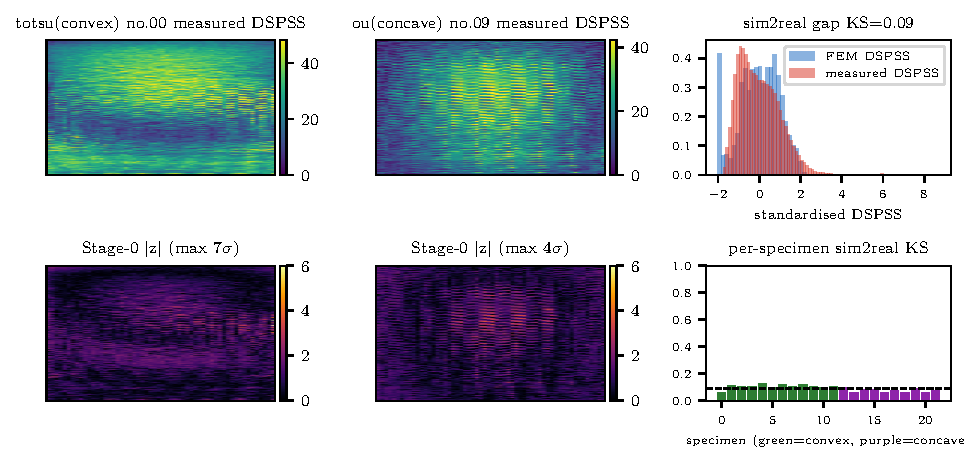
\includegraphics[height=2.2cm]{tsa_sim2real.pdf}\\{\scriptsize Sim-to-real (TSA)}
\end{column}
\begin{column}{0.32\textwidth}\centering
  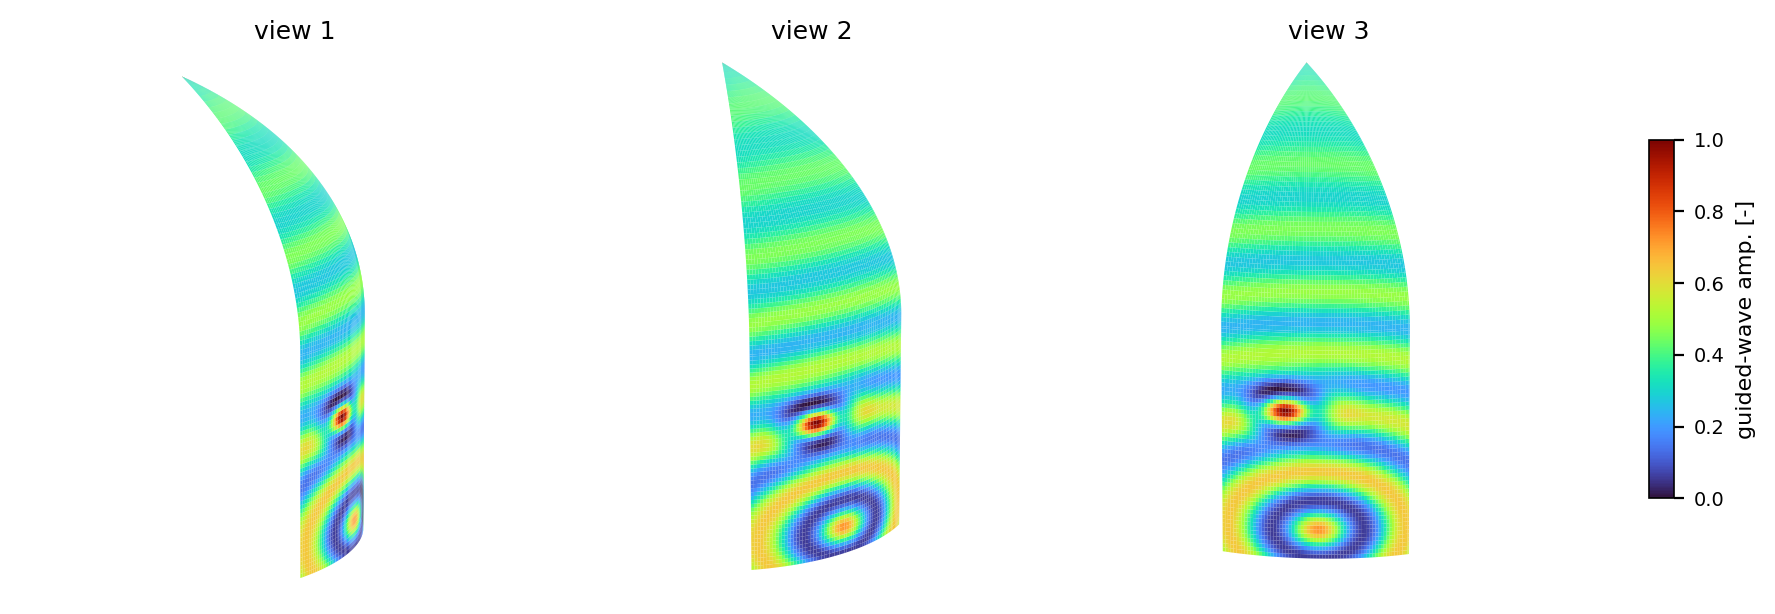
\includegraphics[height=2.2cm]{fairing_3d.png}\\{\scriptsize Payload-fairing SHM}
\end{column}
\end{columns}
\vspace{0.2em}
{\footnotesize\itshape Preliminary; not part of the published results.}
\end{frame}

% ---------------------------------------------------------------------
\begin{frame}{Acknowledgements}
\note{Thank the co-authors and JAXA, then invite questions.}
\begin{itemize}
  \item Conducted in collaboration with \textbf{JAXA} (Research \& Development Directorate, Research Unit IV).
  \item Co-authors at \textbf{Keio University}, \textbf{Nagoya University}, and \textbf{JAXA}.
  \item Built on the FEA-generated CFRP interstage dataset of the prior study~\cite{kojima}.
\end{itemize}
\vspace{0.8em}
\centering Thank you for your attention --- questions welcome.
\end{frame}

% ---------------------------------------------------------------------
\begin{frame}[allowframebreaks]{References}
\renewcommand*{\bibfont}{\tiny}
\printbibliography[heading=none]
\end{frame}

% =====================================================================
%  APPENDIX — difference-data details (course-1 / 差分データ)
% =====================================================================
\appendix

\begin{frame}
\vfill
\centering
{\usebeamercolor[fg]{title}\Large\bfseries Appendix}
\vfill
\end{frame}

% ---------------------------------------------------------------------
\begin{frame}{Appendix: difference-data construction}
\begin{columns}[T]
\begin{column}{0.5\textwidth}
Raw DSPSS near a hole is dominated by geometric stress concentration.
We remove it by a per-specimen \textbf{difference}:
\[
  \text{Difference} = \underbrace{\text{Original (defect)}}_{\text{damaged}}
  - \underbrace{\text{Reference (no defect)}}_{\text{pristine}} .
\]
The residual isolates the defect-induced perturbation, independent of the
hole's baseline field.
\end{column}
\begin{column}{0.5\textwidth}
  \centering
  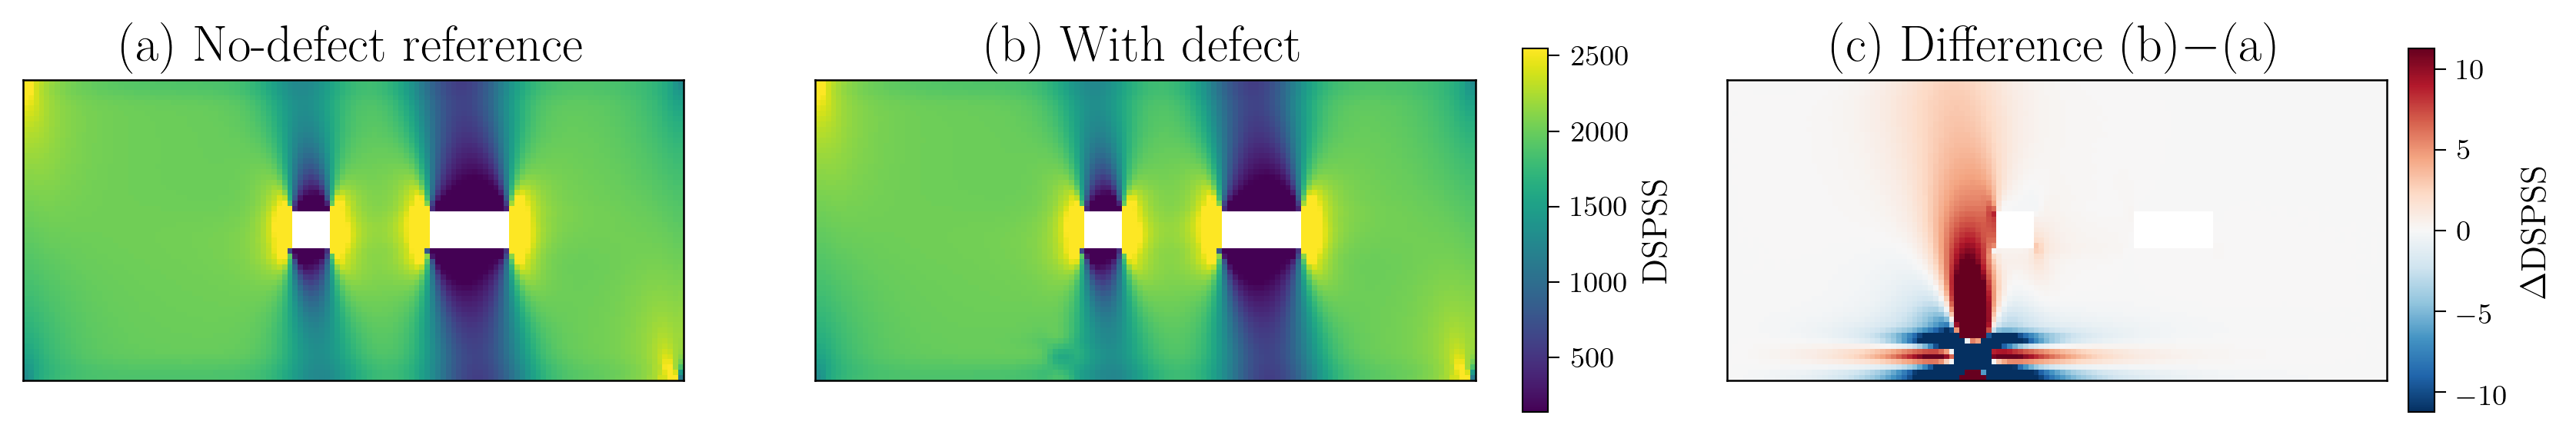
\includegraphics[width=\linewidth]{diff_clean.png}\\
  {\scriptsize With-defect $-$ no-defect reference $=$ difference field (defect localized).}
\end{column}
\end{columns}
\end{frame}

% ---------------------------------------------------------------------
\begin{frame}{Appendix: Z-score normalization}
\begin{columns}[T]
\begin{column}{0.5\textwidth}
The difference field is standardized per node (Z-score):
\[
  \hat\sigma = \frac{\sigma - \mu}{s}.
\]
\begin{itemize}
  \item equalizes magnitude across regions/specimens;
  \item improves \textbf{depth-direction} (layer) discrimination;
  \item keeps the network NDT-admissible (coordinate/stress only).
\end{itemize}
\end{column}
\begin{column}{0.5\textwidth}
  \centering
  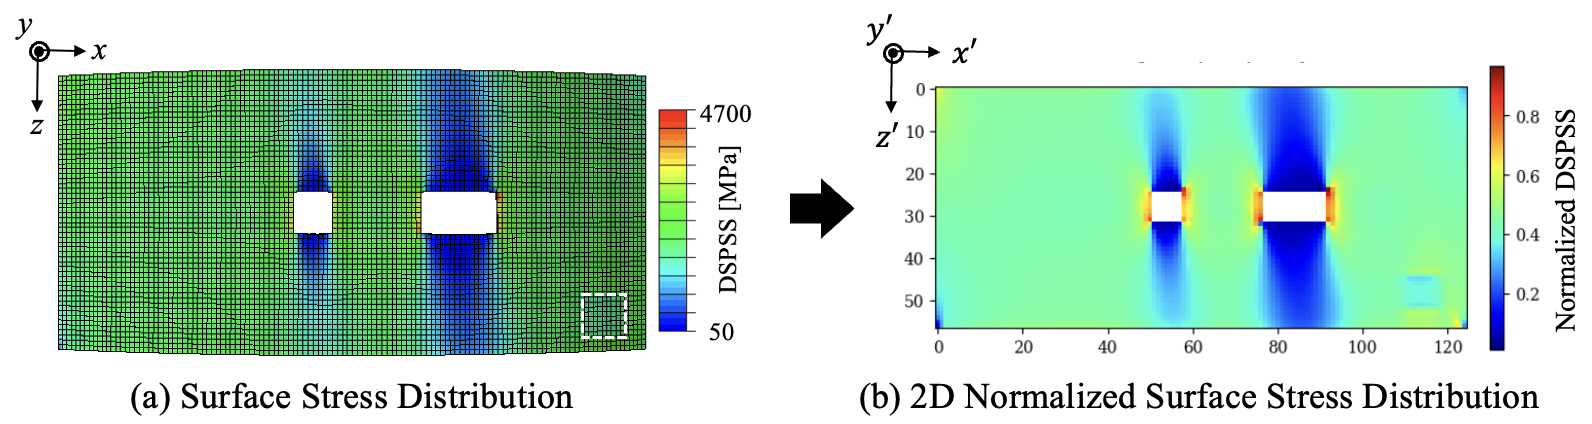
\includegraphics[width=\linewidth]{dspss_normalized.png}\\
  {\scriptsize Normalized DSPSS input (paper figure).}
\end{column}
\end{columns}
\end{frame}

% ---------------------------------------------------------------------
\begin{frame}{Appendix: DSPSS profile around the defect}
\begin{columns}[T]
\begin{column}{0.46\textwidth}
The difference-DSPSS shows a pronounced \textbf{stress valley} at the defect
centre; its depth and width encode the insertion layer (ply-angle dependence).
\end{column}
\begin{column}{0.54\textwidth}
  \centering
  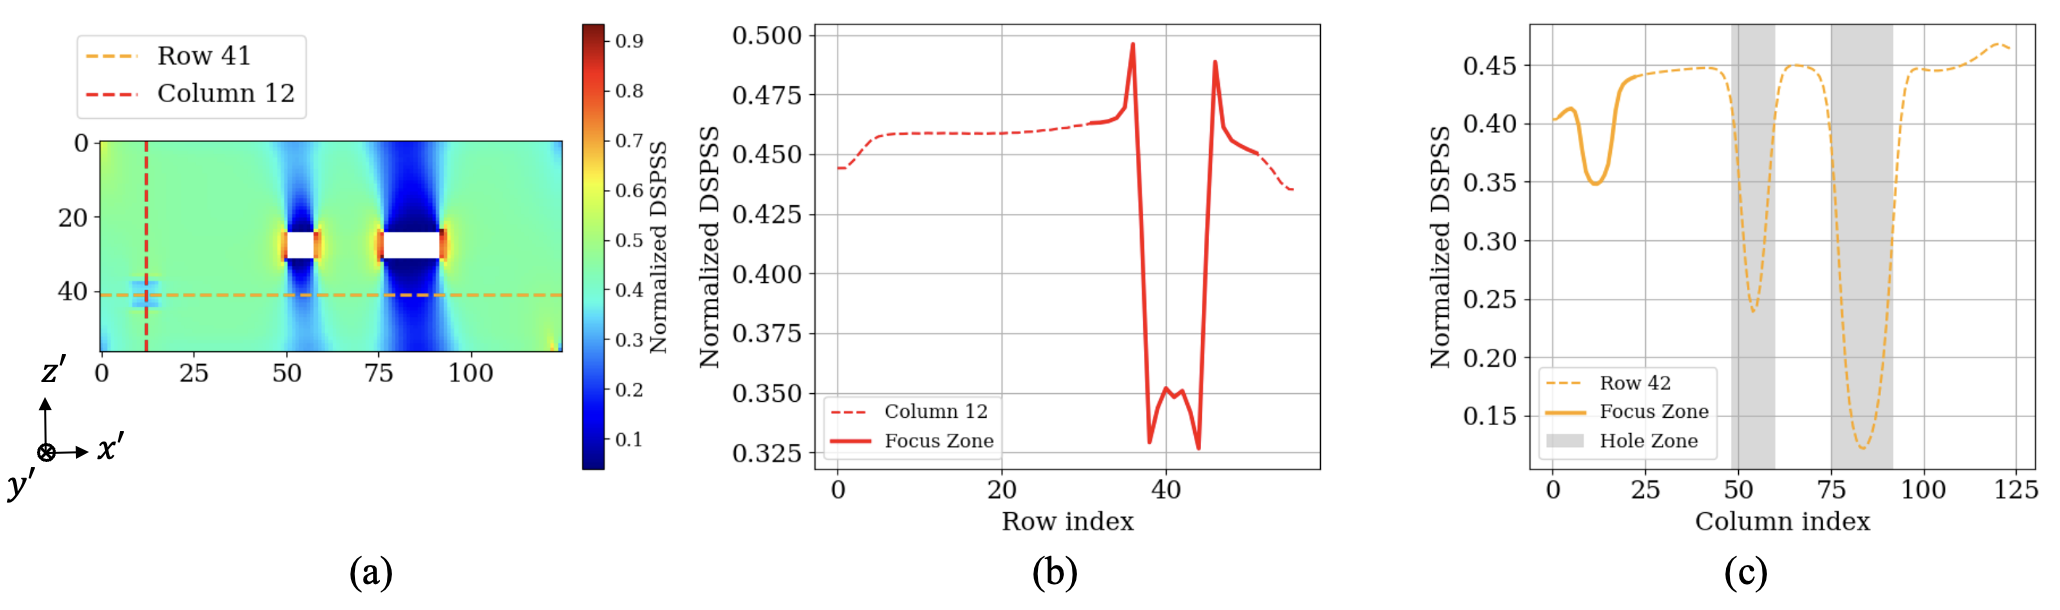
\includegraphics[width=\linewidth]{dspss_profile.png}\\
  {\scriptsize Profile of the normalized DSPSS across the defect (paper figure).}
\end{column}
\end{columns}
\end{frame}

% ---------------------------------------------------------------------
\begin{frame}{Appendix: evaluation metrics}
\begin{itemize}
  \item \textbf{$R$} --- in-plane (planar) F1 score for defect vs.\ non-defect at the
        correct location.
  \item \textbf{$P_{\mathrm{gauss}}$} --- depth-direction score: Gaussian-weighted
        ($\sigma = 2$ layers) credit for predicting the correct or a near-correct
        insertion layer.
  \item \textbf{TDPS} (Total Defect Prediction Score) $= \tfrac{1}{2}\,(R + P_{\mathrm{gauss}})$.
  \item \textbf{macro-F1} --- unweighted mean F1 over all 19 classes (the headline metric).
\end{itemize}
\vspace{0.4em}
These quantify in-plane localization ($R$), depth/layer accuracy ($P_{\mathrm{gauss}}$),
and their combination (TDPS), complementing the class-level macro-F1.
\end{frame}

% ---------------------------------------------------------------------
\begin{frame}{Appendix: what the Stage-0 screen keys on (one case)}
\note{Backup for a likely question --- what does the per-node screen actually respond to. On real 4x4-defect specimens we decompose a case. Two robust facts. First, where: the defect nodes rank in the top about zero-point-two percent by score, per-case AUROC about 0.998, aggregated over two hundred specimens, not cherry-picked. Second, which way: ninety-eight to one hundred percent of the defect-node deviations are negative --- the screen keys on a local stress valley, which is exactly the thermoelastic signature of a sub-surface defect. The honest caveats: the absolute z magnitudes are inflated because the per-node sigma is tiny on a z-scored field, so I only quote rank and sign, never N-sigma; and top-K precision is below one because the hole-edge concentration also deviates strongly --- which is precisely why we difference-normalize the input before precise localization.}
\begin{columns}[T]
\begin{column}{0.6\textwidth}
  \centering
  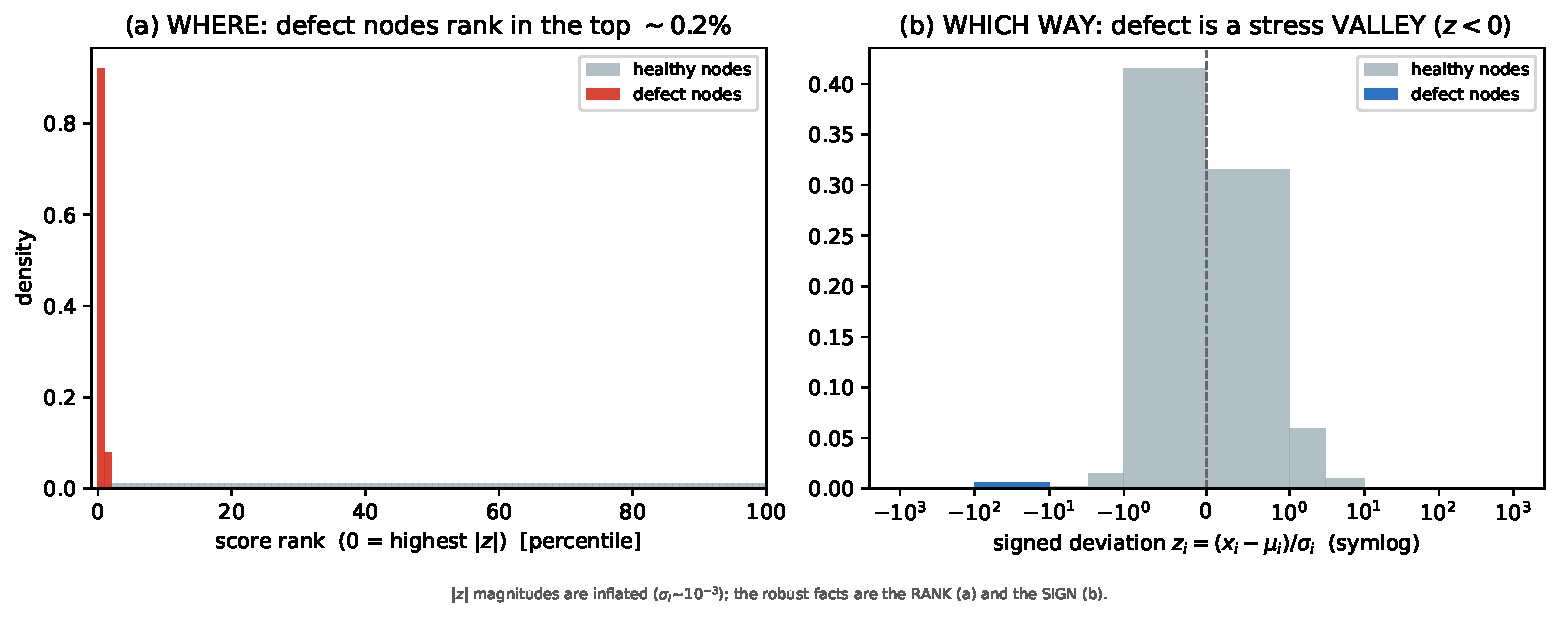
\includegraphics[width=\linewidth]{../paper_figs/stage0_case_study.pdf}
\end{column}
\begin{column}{0.4\textwidth}\small
Real 4$\times$4 specimens, per-node $s_i=|x_i-\mu_i|/\sigma_i$:
\begin{itemize}\small
  \item \textbf{Where:} defect nodes rank \textbf{top $\sim$0.2\%};
        per-case \best{AUROC $0.998$} (200 specimens).
  \item \textbf{Which way:} \textbf{98--100\% negative} deviation
        $\Rightarrow$ a \emph{stress valley} (thermoelastic signature).
\end{itemize}
\begin{block}{Honest limits}
\scriptsize
$|z|$ magnitudes inflated ($\sigma_i\!\sim\!10^{-3}$) --- quote rank/sign, not
``$N\sigma$''. precision@K $<1$: the hole edge also deviates $\Rightarrow$ the
reason we \emph{difference-normalize} before precise localization.
\end{block}
\end{column}
\end{columns}
\end{frame}

\end{document}
